\documentclass{beamer}
%
% Choose how your presentation looks.
%
% For more themes, color themes and font themes, see:
% http://deic.uab.es/~iblanes/beamer_gallery/index_by_theme.html
%
\mode<presentation>
{
  \usetheme{default}      % or try Darmstadt, Madrid, Warsaw, ...
  \usecolortheme{beaver} % or try albatross, beaver, crane, ...
  \usefonttheme{default}  % or try serif, structurebold, ...
  \setbeamertemplate{navigation symbols}{}
  \setbeamertemplate{caption}[numbered]
} 

\usepackage[english]{babel}
\usepackage[utf8x]{inputenc}
\usepackage{hyperref}
\hypersetup{
    colorlinks=true,
    linkcolor=blue,
    filecolor=magenta,      
    urlcolor=blue,
}

\title[Control Interfaces]{Control Interfaces}
\author{Andrés Pérez}
\institute{Digital Lutherie\\Master en Música para Experiencias del Entretenimiento\\ENTI-UB}
\date{2018/2019}

\newcommand\blfootnote[1]{%
  \begingroup
  \renewcommand\thefootnote{}\footnote{#1}%
  \addtocounter{footnote}{-1}%
  \endgroup
}

\AtBeginSection[]
{
\begin{frame}{Outline}
    \tableofcontents[currentsection] 
\end{frame}
}

\begin{document}

\begin{frame}
  \titlepage
\end{frame}



\begin{frame}{Outline}
 \tableofcontents
\end{frame}

%%%%%%%%%%%%%%%%%%%%%%%%%%%%%%%%%%%%%%%%%%%%%%%%%%
%%%%%%%%%%%%%%%%%%%%%%%%%%%%%%%%%%%%%%%%%%%%%%%%%%
%%%%%%%%%%%%%%%%%%%%%%%%%%%%%%%%%%%%%%%%%%%%%%%%%%
\section{Control Interfaces}

\begin{frame}{Control Interfaces}
    \begin{figure}[h]
        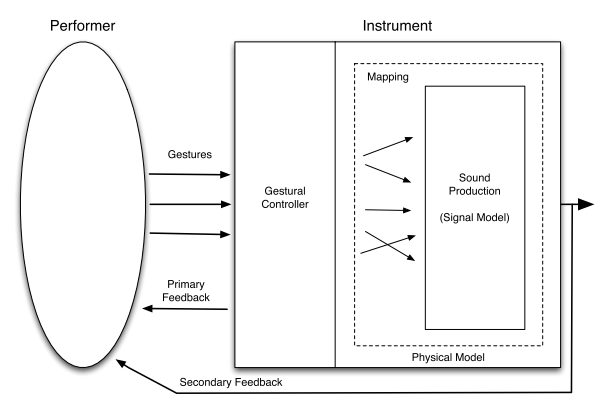
\includegraphics[width=0.9\textwidth]{instrument_scheme.png}\blfootnote{Wanderley, M. M. (2001). Performer-Instrument Interaction: Applications to Gestural Control of Sound Synthesis. PhD thesis, University Paris 6.}
    \end{figure}
\end{frame}


%%%%%%%%%%%%%%%%%%%%%%%%%%%%%%%%%%%%%%%%%%%%%%%%%%
\subsection{Definition}

\begin{frame}{Control Interfaces - Definition}
    (Tentative definition)\\
    \vspace{5mm}
    The \textit{Control Interface} (also called \textit{Gestural Controller}, \textit{Instrument Body}, \textit{Input Device}, \textit{Physical Interface}, or just \textit{Interface} or \textit{Controller}) is the part of the instrument with which the performer interacts through gestures. 
\end{frame}

\begin{frame}{Control Interfaces - Definition}
    In the case of DMIs, the control interface can be \textbf{anything} that provides the user a way to interact, and it is capable to quantify this interaction in a digital way, to be understood by a microprocessor.
\end{frame}

\begin{frame}{Control Interfaces - Definition}
    \textit{"The controller component can typically be a simple computer mouse, a computer keyboard, a MIDI keyboard or a MIDI fader box, but with the use of sensors and appropriate analogue to digital converters, any control signal coming from the outside (i.e. the performer, but also the audience or the environment – as in the case of interactive installations) can be converted into control messages understandable by the digital system. Changes in motion, pressure, velocity, light, gravity, skin conductivity or muscle tension, almost anything, can now become a ‘music controller’."}\footnote{Jordà, S. (2007). Interactivity and live computer music. Computer Music Journal.}
\end{frame}

\begin{frame}{Control Interfaces - Definition}
    (Anticipated conclusion)\\
    \vspace{5mm}
    \textit{“Any input device can become a good or a bad choice depending on the context, the parameter to control, or the performer who will be using it”}\footnote{Jordà, S. (2007). Interactivity and live computer music. Computer Music Journal.}
\end{frame}

%%%%%%%%%%%%%%%%%%%%%%%%%%%%%%%%%%%%%%%%%%%%%%%%%%
\subsection{Taxonomy}

\begin{frame}{Control Interfaces - Taxonomy}
    Wanderley's classification:\footnote{Wanderley, M. M. (2001). Gestural Control of Music. International Workshop Human Supervision and Control in Engineering and Music.} 
    \begin{itemize}
        \item Instrument-like Controllers
        \item Augmented Controllers
        \item Alternate Controllers
    \end{itemize}
\end{frame}

\begin{frame}{Control Interfaces - Taxonomy}
   Instrument-like Controllers\\
   \vspace{5mm}
   \begin{itemize}
        \item The controller design tries to faithfully replicate an existing acoustic instrument.
        \item Electronic versions of traditional instruments.
        \item Subcategory: Instrument-inspired controllers
\end{itemize}
\end{frame}

\begin{frame}{Control Interfaces - Taxonomy}
    \begin{figure}[h]
        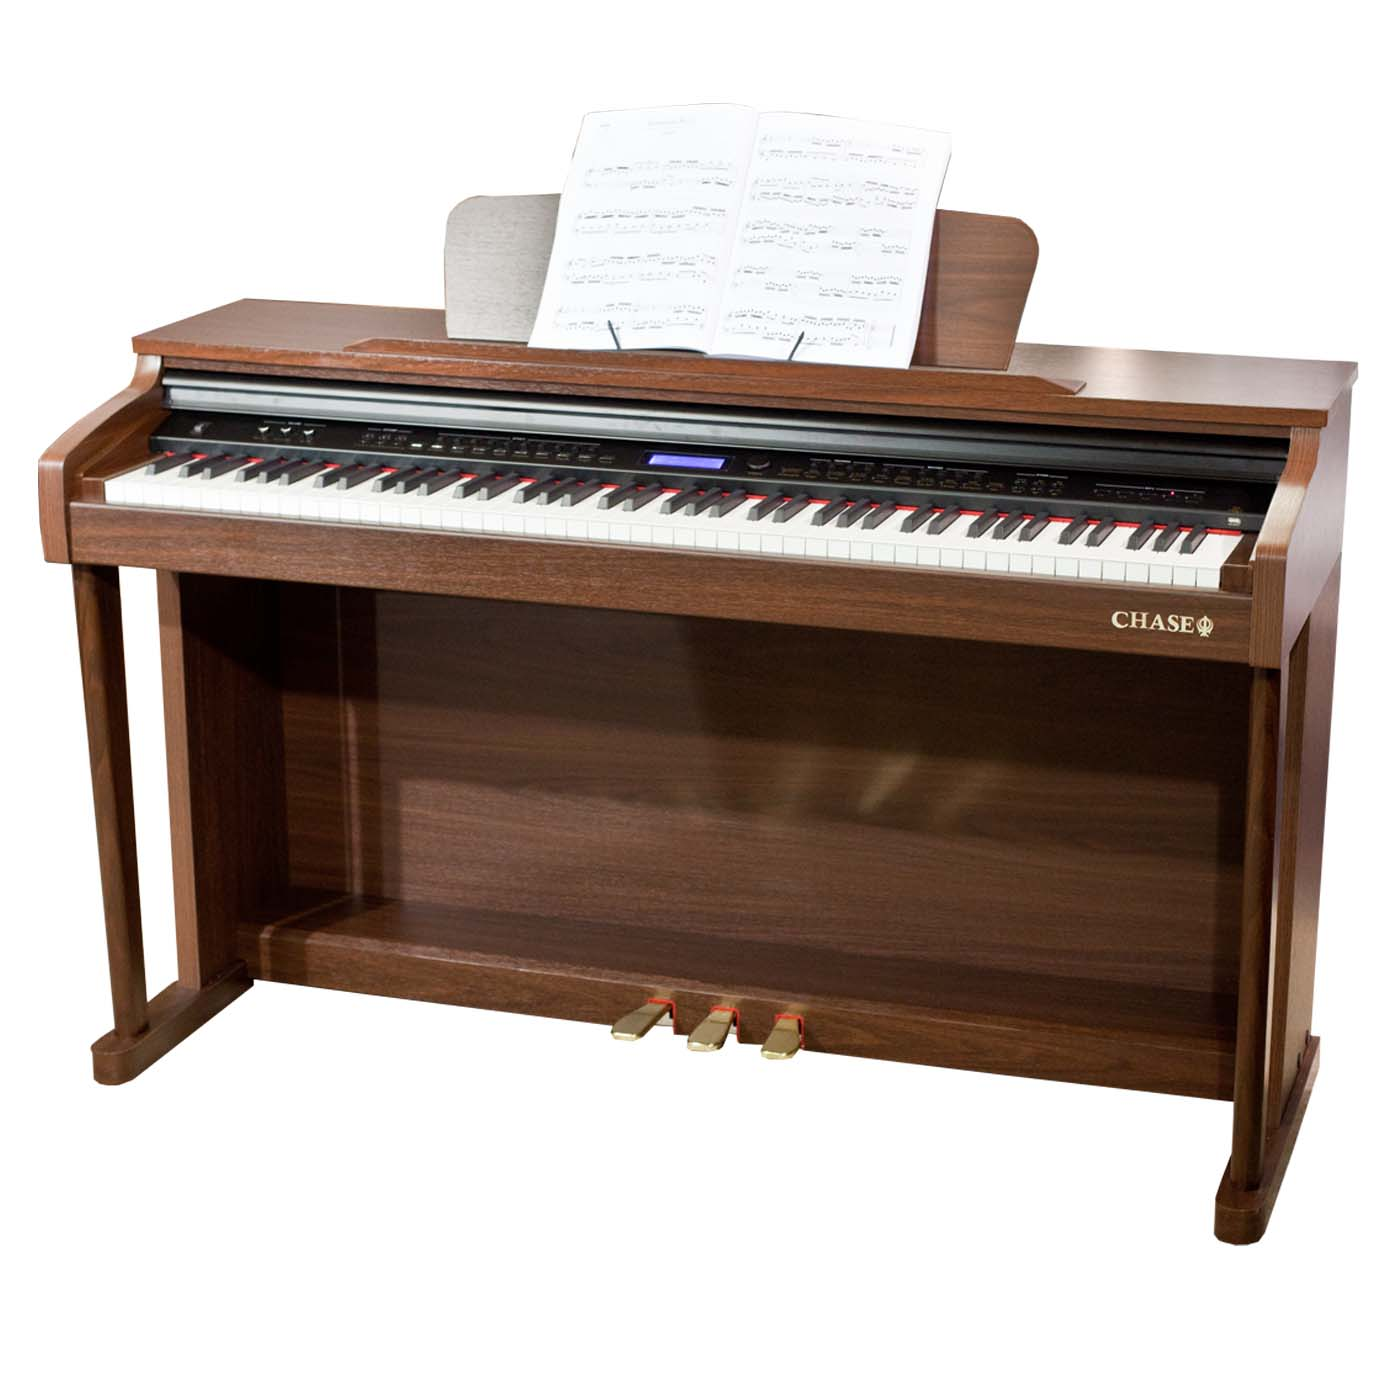
\includegraphics[width=0.5\textwidth]{epiano.jpg}\blfootnote{By Pianomangeorge - Own work, CC BY-SA 4.0, https://commons.wikimedia.org/w/index.php?curid=46988058}
    \end{figure}
\end{frame}

\begin{frame}{Control Interfaces - Taxonomy}
    \begin{figure}[h]
        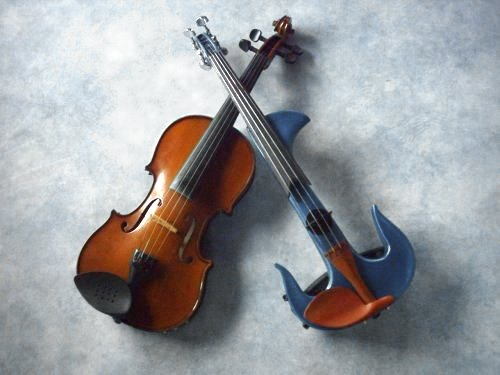
\includegraphics[width=0.9\textwidth]{eviolin.jpeg}
    \end{figure}
\end{frame}

\begin{frame}{Control Interfaces - Taxonomy}
    \begin{figure}[h]
        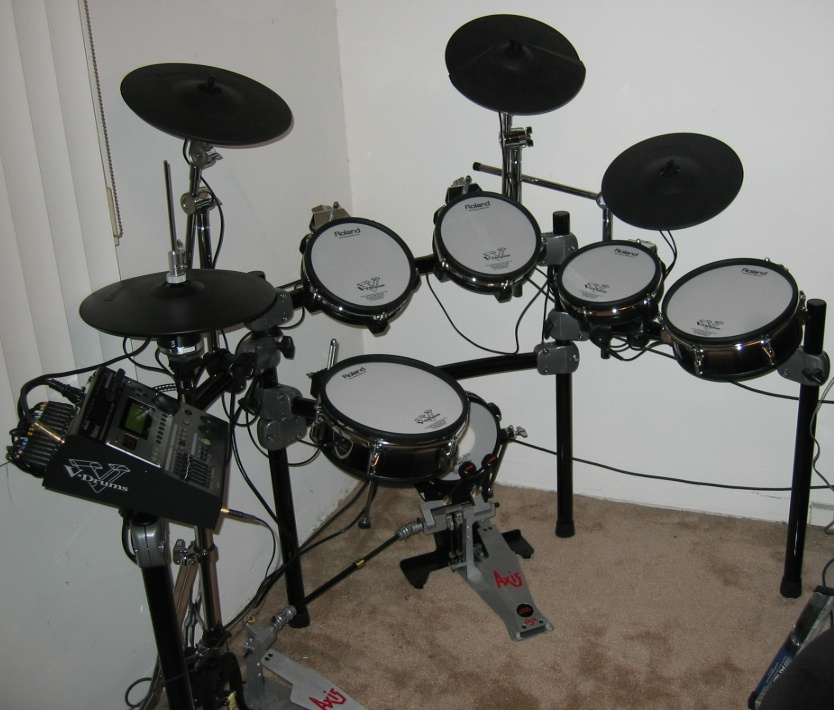
\includegraphics[width=0.75\textwidth]{edrums.jpg}
    \end{figure}
\end{frame}

\begin{frame}{Control Interfaces - Taxonomy}
    \begin{figure}[h]
        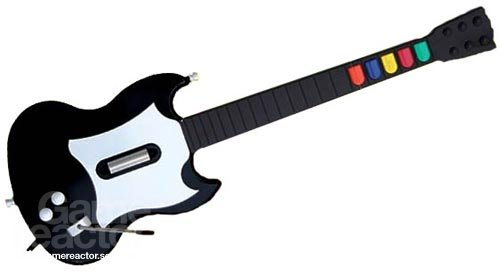
\includegraphics[width=\textwidth]{guitarhero.jpg}\blfootnote{GameReactor,  https://www.gamereactor.eu/images/?productid=200\&id=97749}
    \end{figure}
\end{frame}

\begin{frame}{Control Interfaces - Taxonomy}
    \begin{figure}[h]
        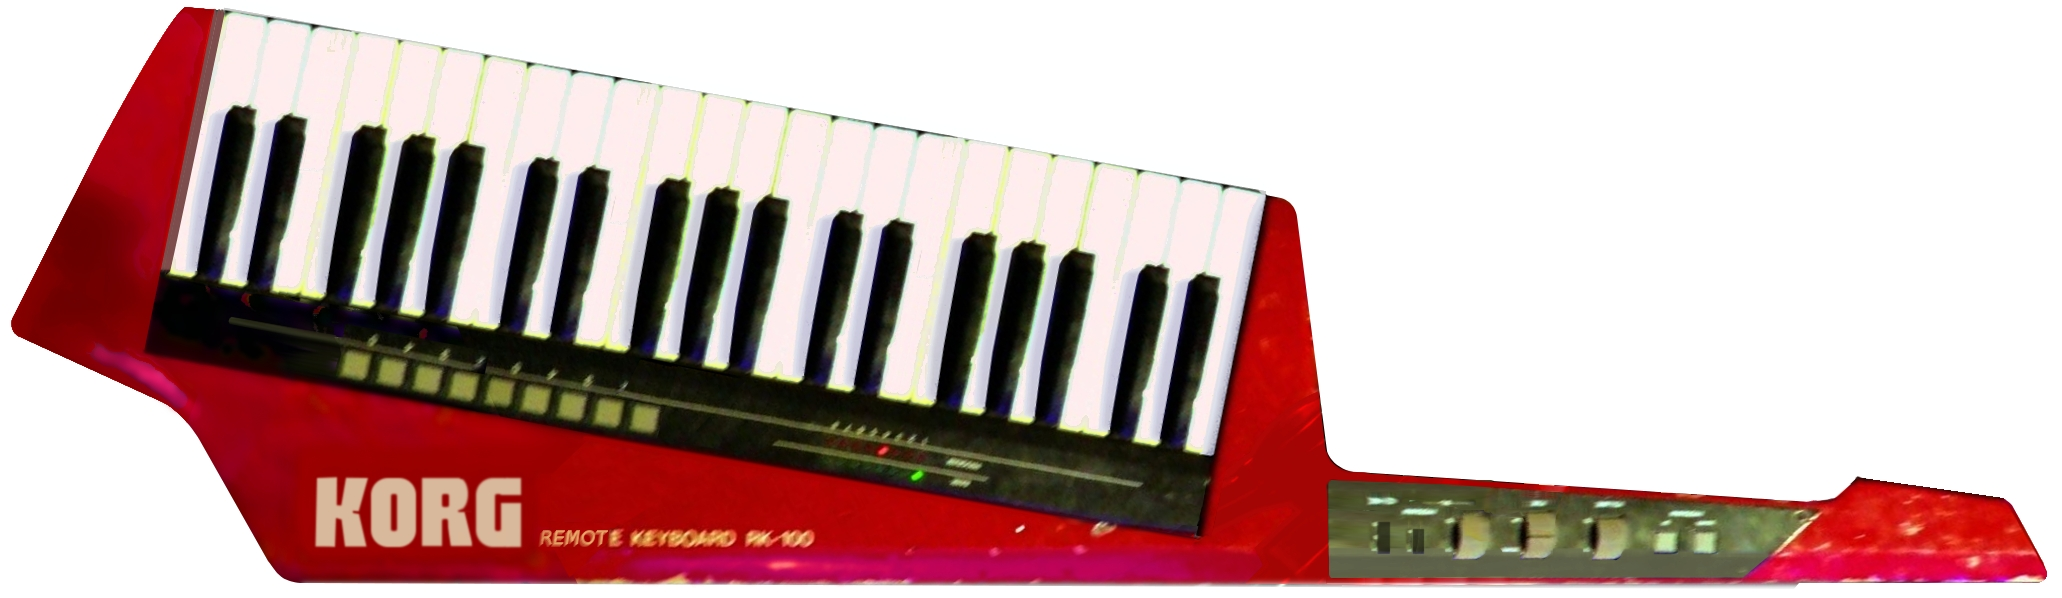
\includegraphics[width=\textwidth]{korgrk100.jpg}\blfootnote{By Keytar.jpg: https://www.flickr.com/photos/tommygunnphotography/derivative work: Clusternote (talk) - Keytar.jpg, CC BY 2.0, https://commons.wikimedia.org/w/index.php?curid=12470544}
    \end{figure}
\end{frame}

\begin{frame}{Control Interfaces - Taxonomy}
    \begin{figure}[h]
        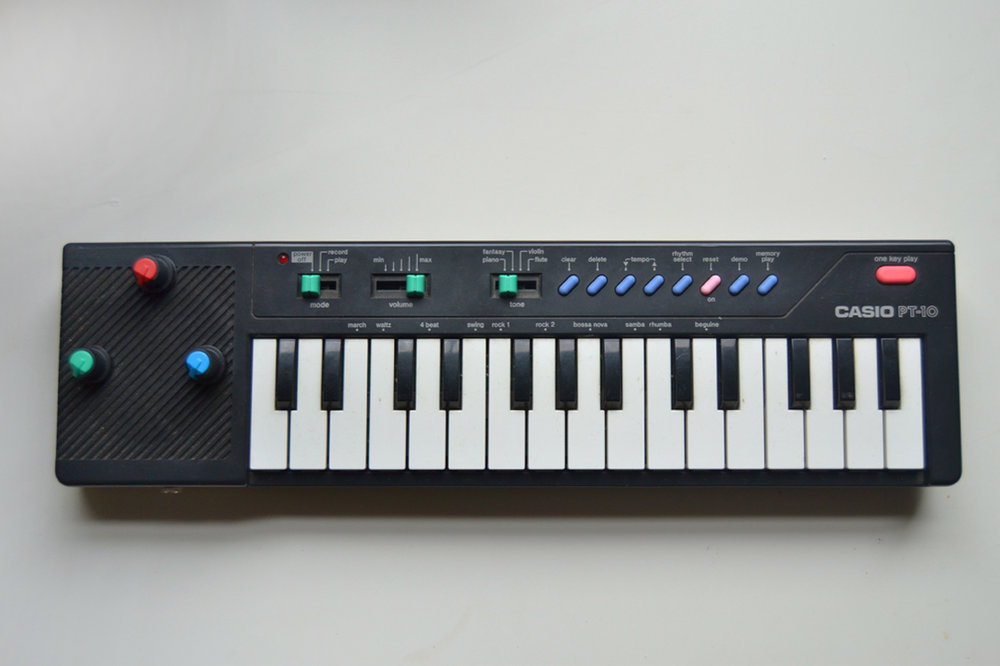
\includegraphics[width=\textwidth]{casiopt10.jpg}\blfootnote{Tasos Stamou,  https://www.tasosstamou.com/shop/casio-pt-10}
    \end{figure}
\end{frame}

\begin{frame}{Control Interfaces - Taxonomy}
    \begin{figure}[h]
        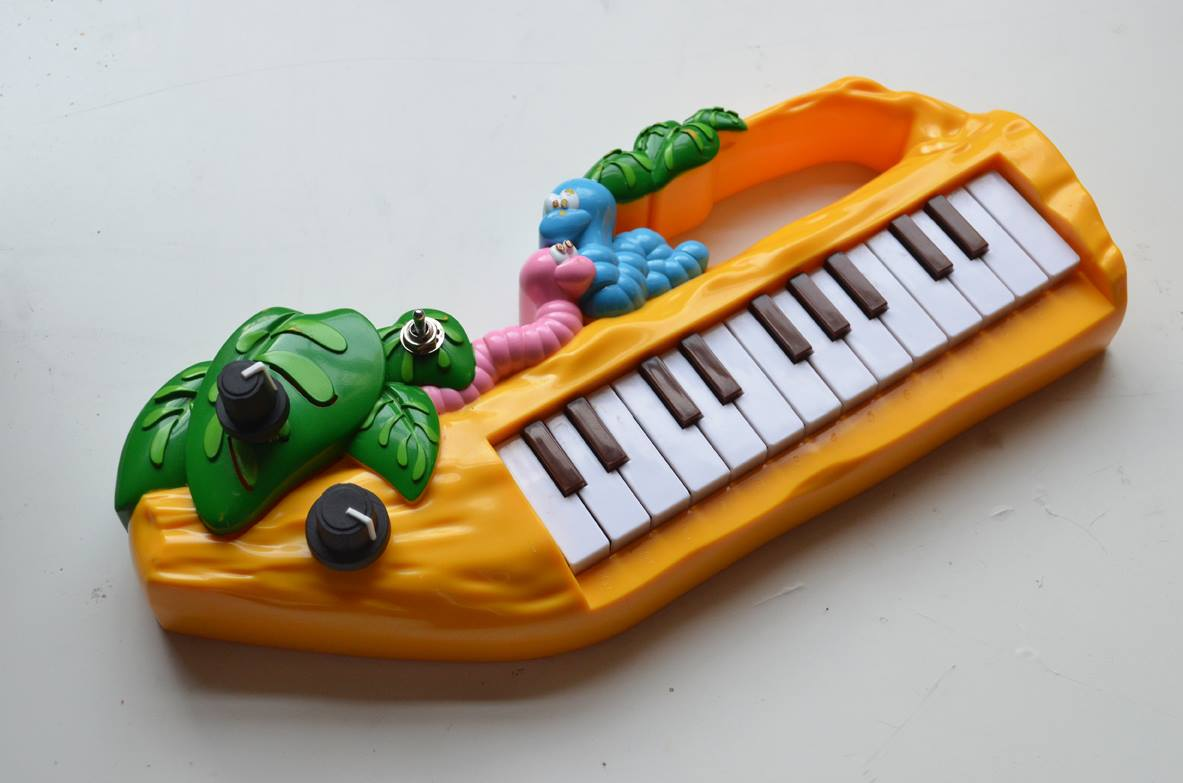
\includegraphics[width=\textwidth]{pianoturtle.jpg}\blfootnote{Tasos Stamou,  https://www.tasosstamou.com/stamouinstruments}
    \end{figure}
\end{frame}

\begin{frame}{Control Interfaces - Taxonomy}
   Augmented Controllers\\
   \vspace{5mm}
   \begin{itemize}
        \item Acoustic instruments with enhanced gesture possibilities due to sensors 
    \end{itemize}
\end{frame}

\begin{frame}{Control Interfaces - Taxonomy}
    Augmented Clarinet by Stelios Manousakis
    \begin{figure}[h]
        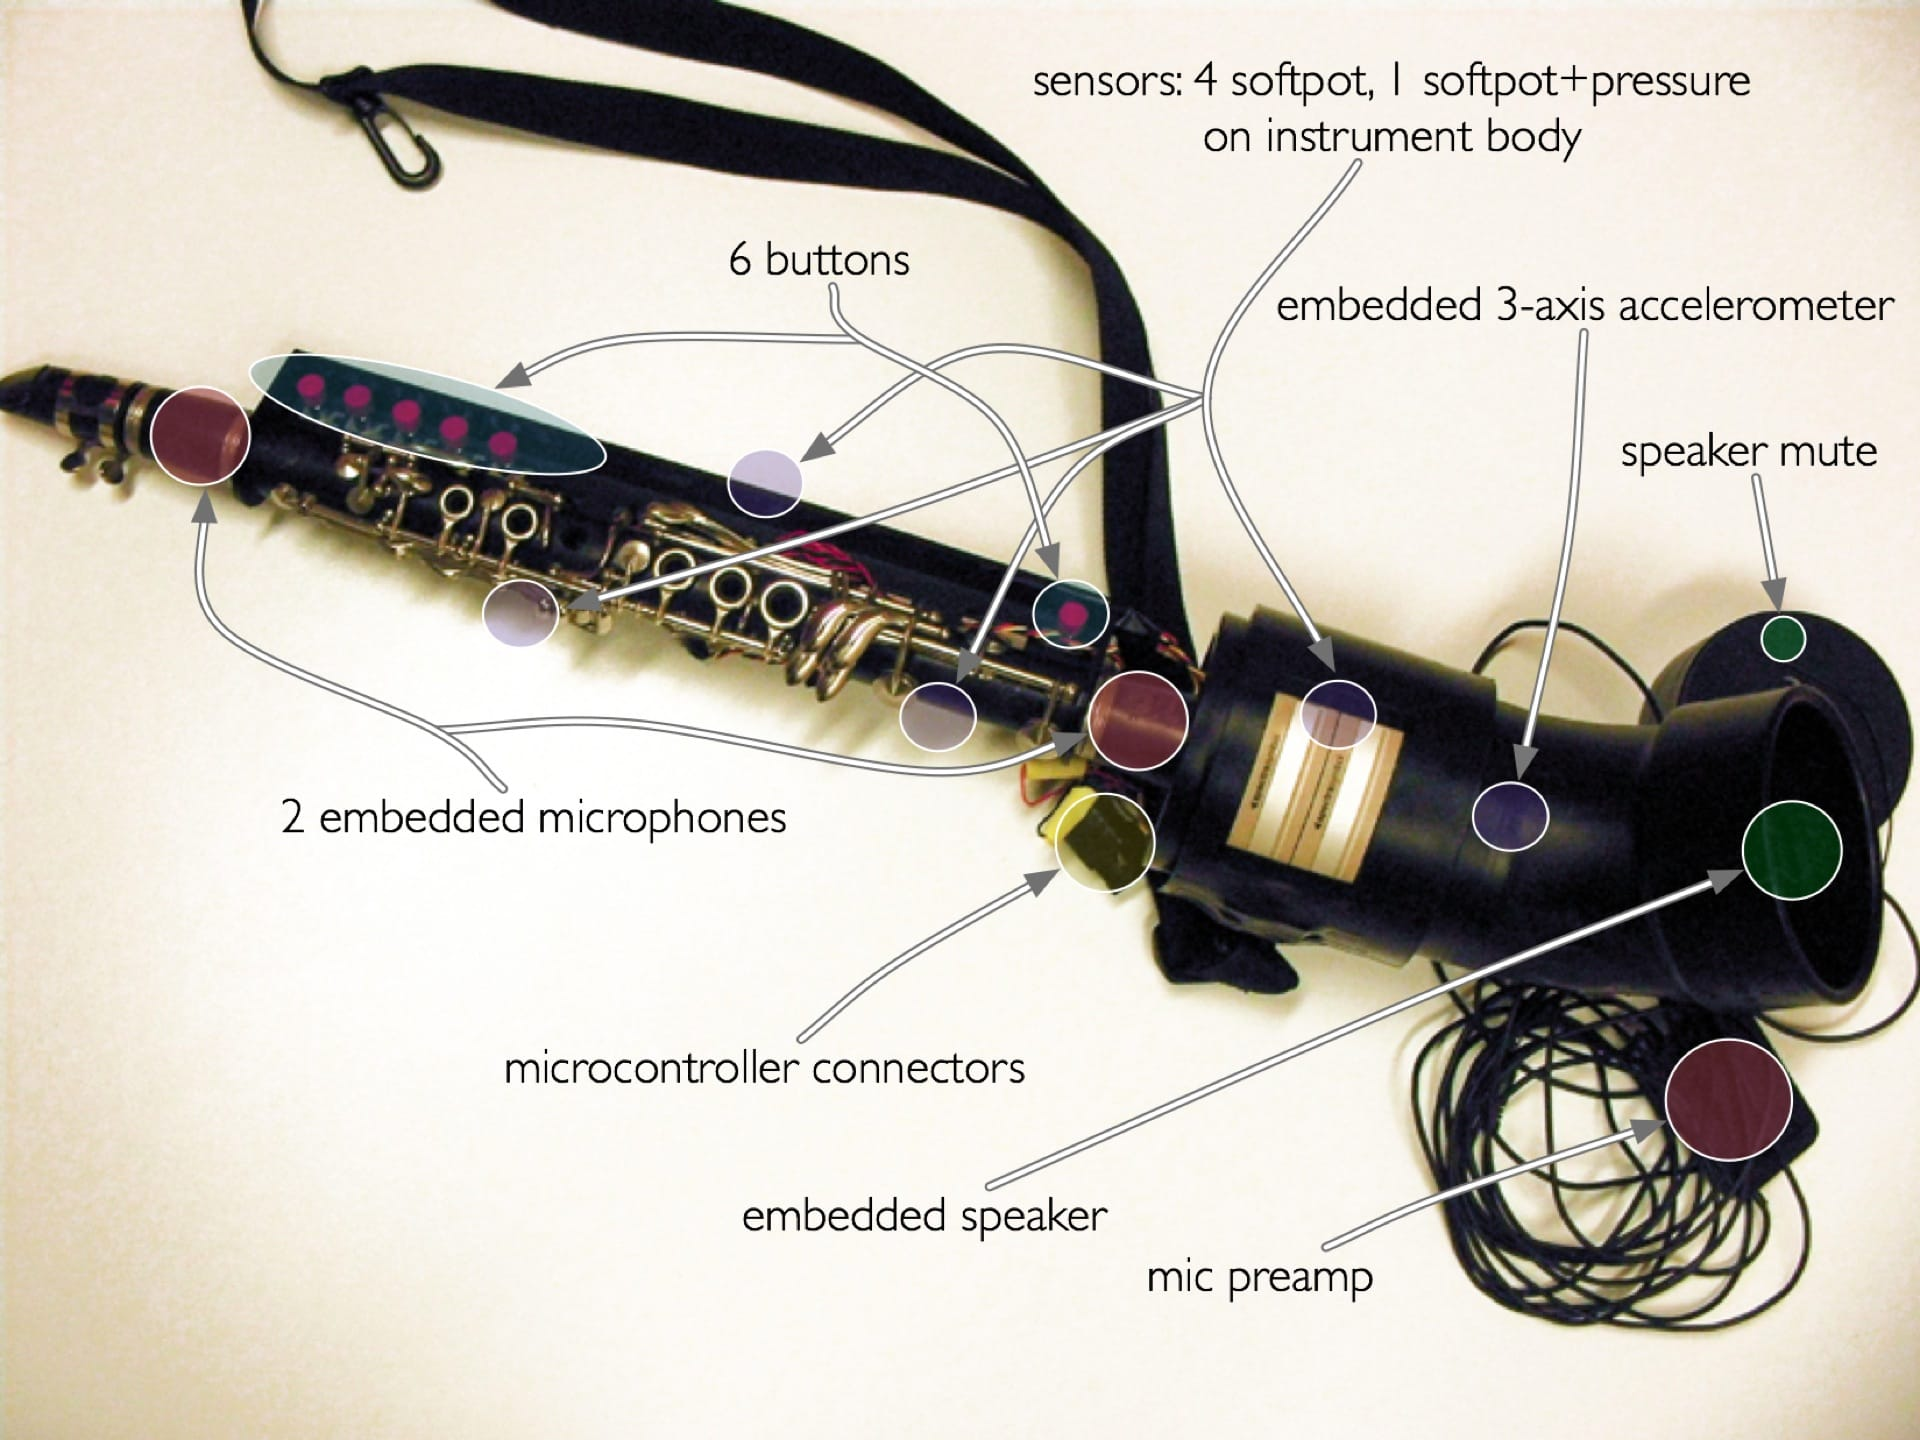
\includegraphics[width=0.7\textwidth]{augmented_clarinet.jpg}\blfootnote{http://modularbrains.net/portfolio/feedback-augmented-sopranino-clarinet/}
    \end{figure}
\end{frame}

\begin{frame}{Control Interfaces - Taxonomy}
    \href{https://www.youtube.com/watch?v=P2syqXx97LE}{Seaboard by ROLI}
    \begin{figure}[h]
        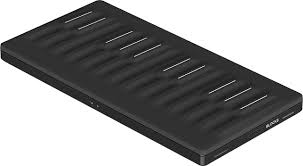
\includegraphics[width=0.7\textwidth]{roli.jpeg}
    \end{figure}
\end{frame}

\begin{frame}{Control Interfaces - Taxonomy}
    \href{https://www.youtube.com/watch?time_continue=153&v=6lfz51eDgfM}{Augmented Piano by A. Veinberg}
    \begin{figure}[h]
        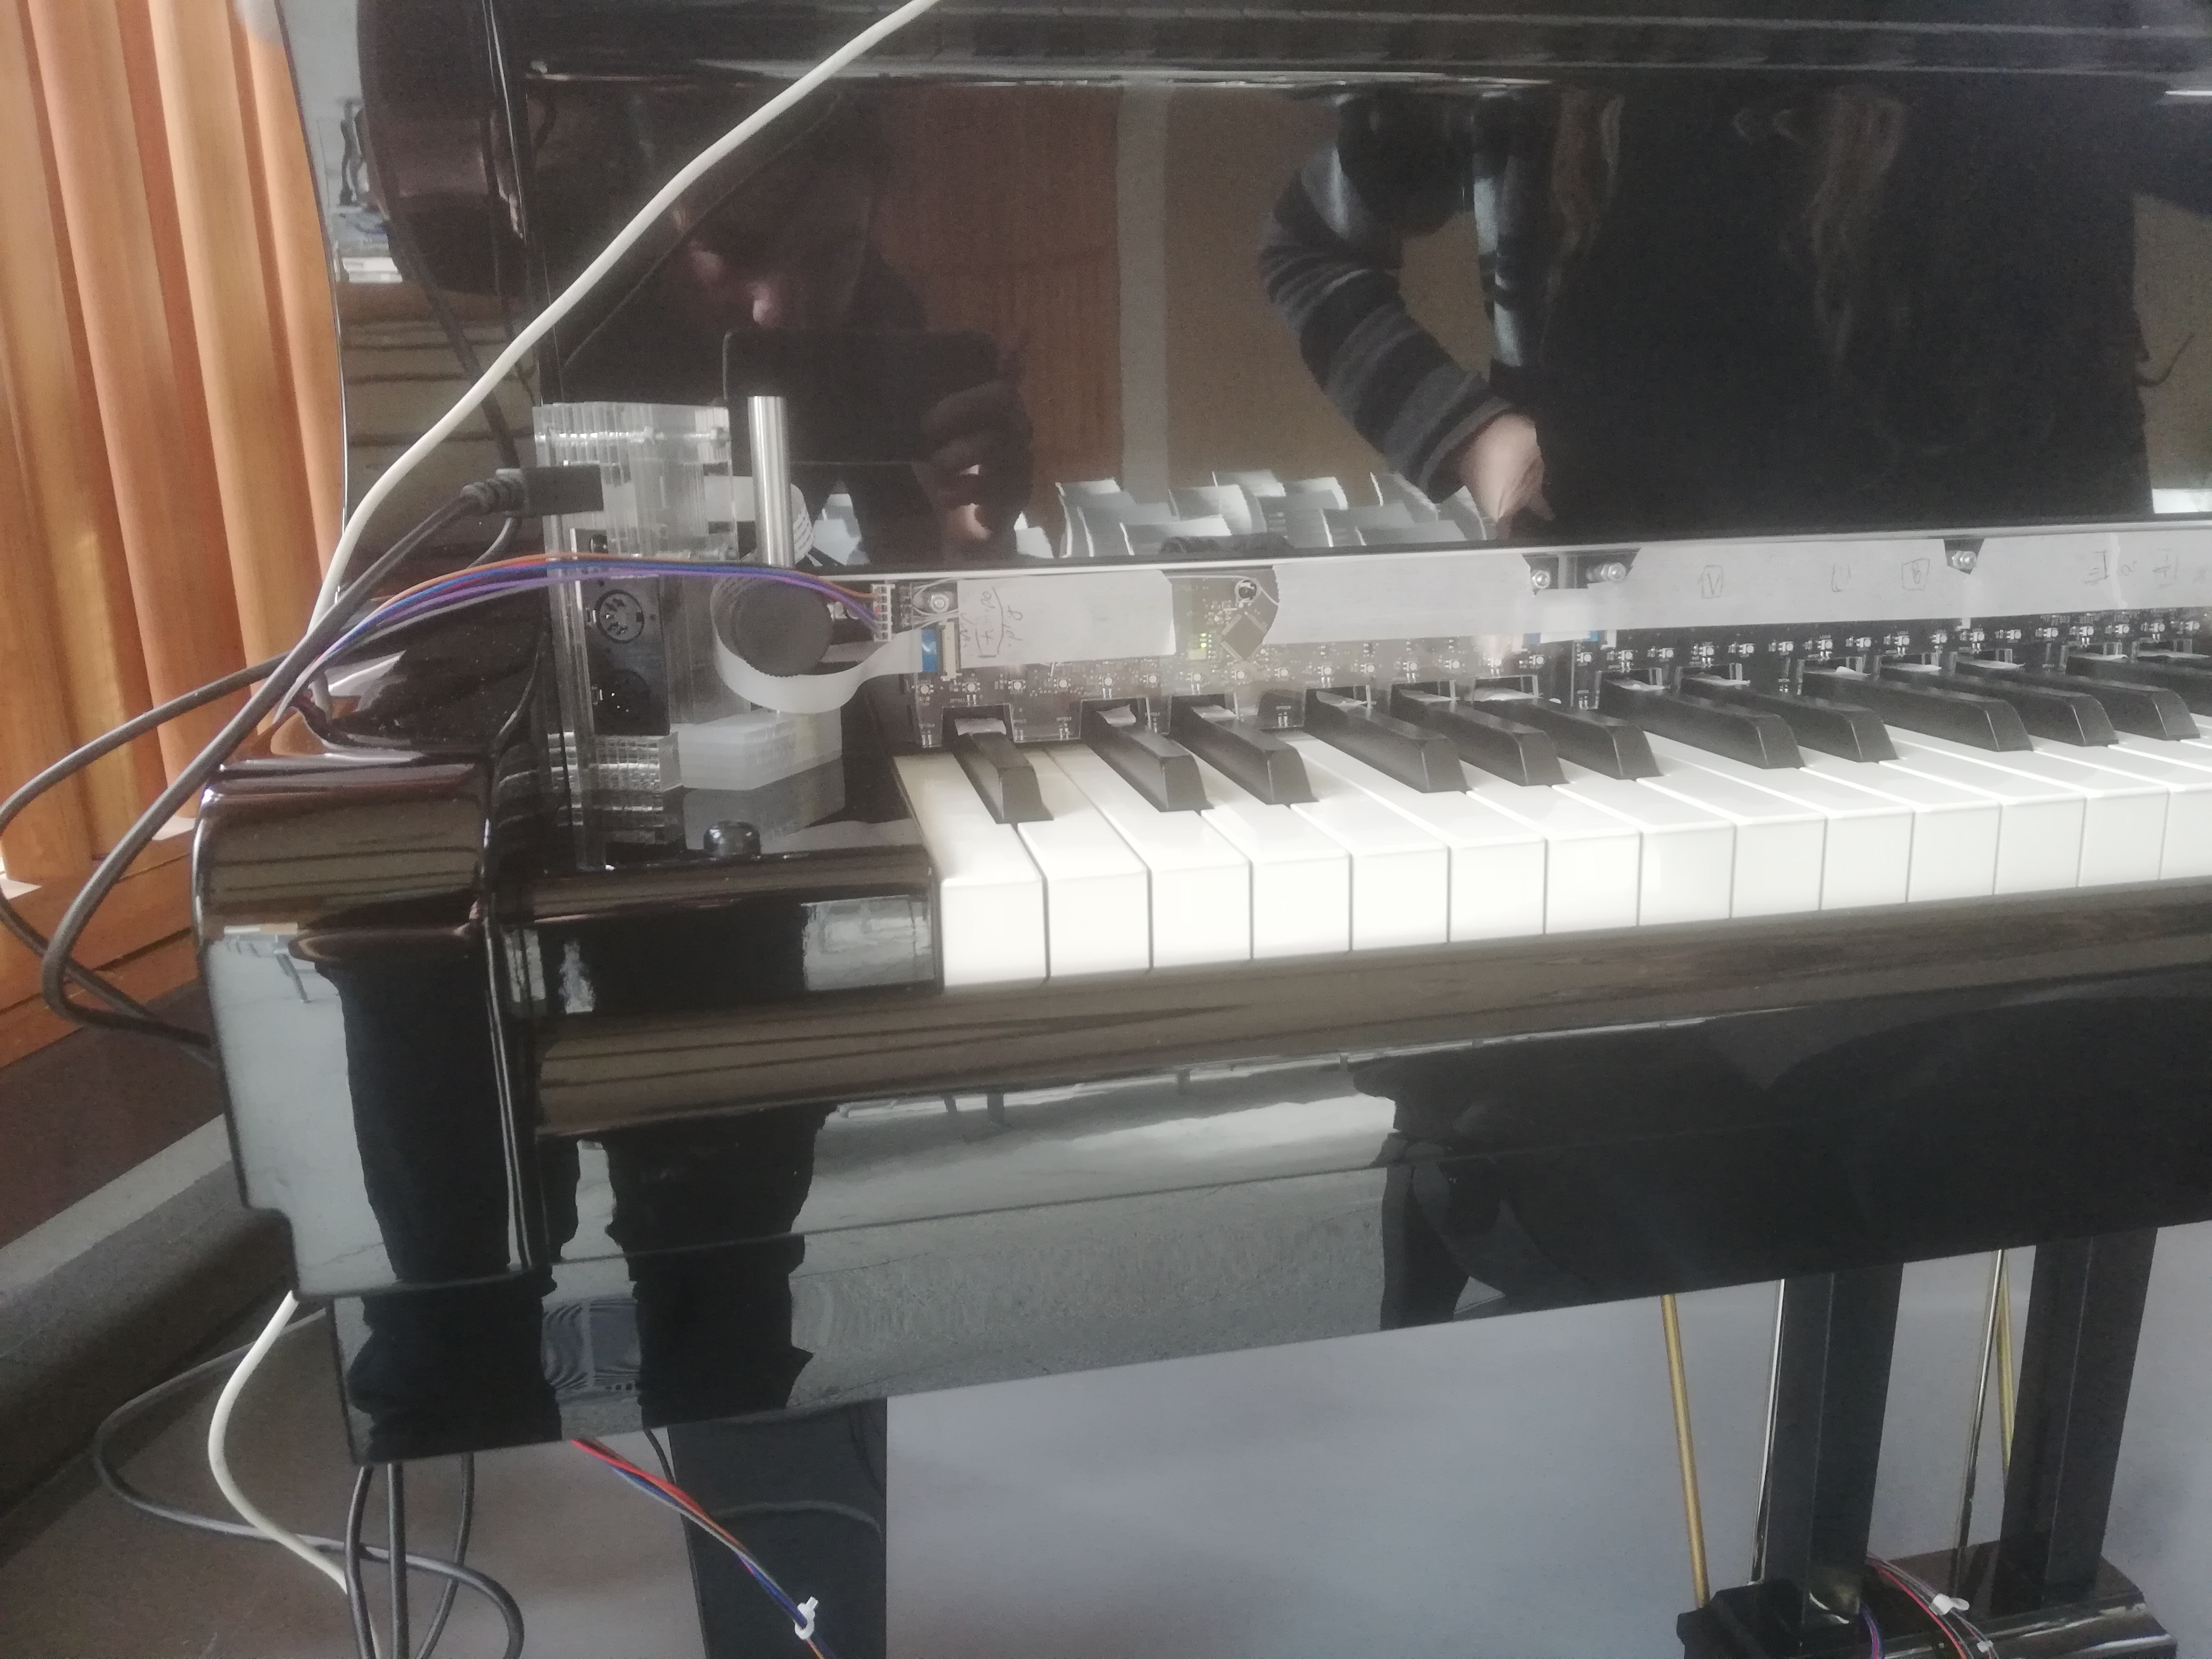
\includegraphics[width=0.9\textwidth]{veinberg.jpg}
    \end{figure}
\end{frame}

\begin{frame}{Control Interfaces - Taxonomy}
    \href{https://www.youtube.com/watch?v=UKRrEdS_SMI}{Augmented Violin by M. Kimura}
    \begin{figure}[h]
        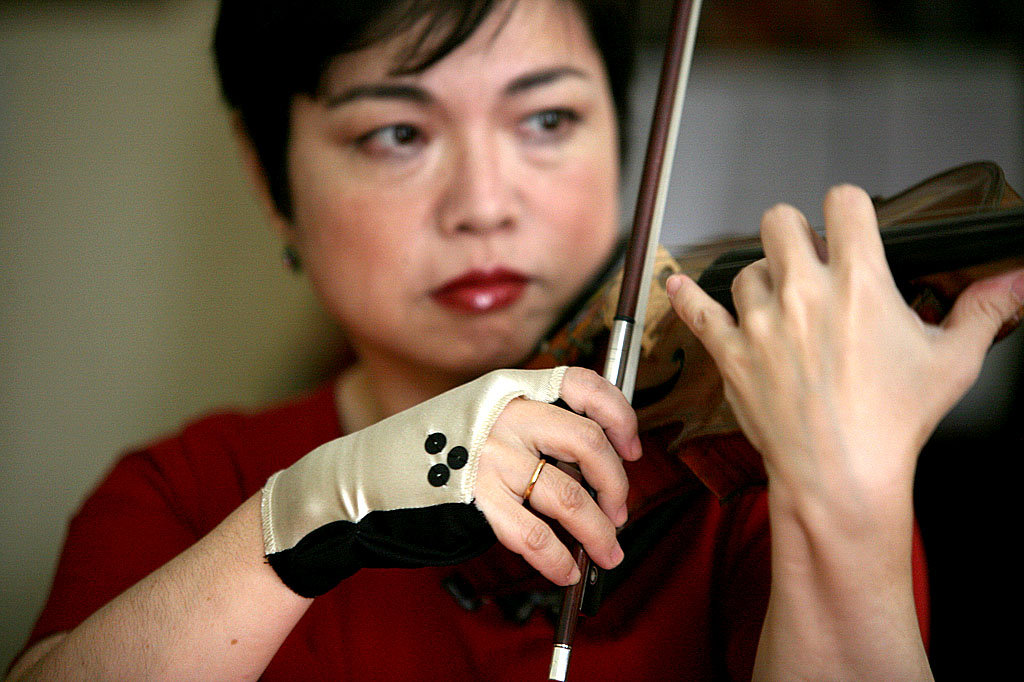
\includegraphics[width=0.9\textwidth]{kimura.jpg}
    \end{figure}
\end{frame}

\begin{frame}{Control Interfaces - Taxonomy}
    \href{https://www.youtube.com/watch?v=Pp-MwmSbOYo}{Does augmented reality produces augmented instruments...?}
\end{frame}

\begin{frame}{Control Interfaces - Taxonomy}
   Alternate Controllers\\
   \vspace{5mm}
   \begin{itemize}
        \item Controllers which are not inspired by existing acoustic instruments 
    \end{itemize}
\end{frame}

\begin{frame}{Control Interfaces - Taxonomy}
    \href{https://www.youtube.com/watch?v=IxMBkwS6Ubg}{Otamatone}
    \begin{figure}[h]
        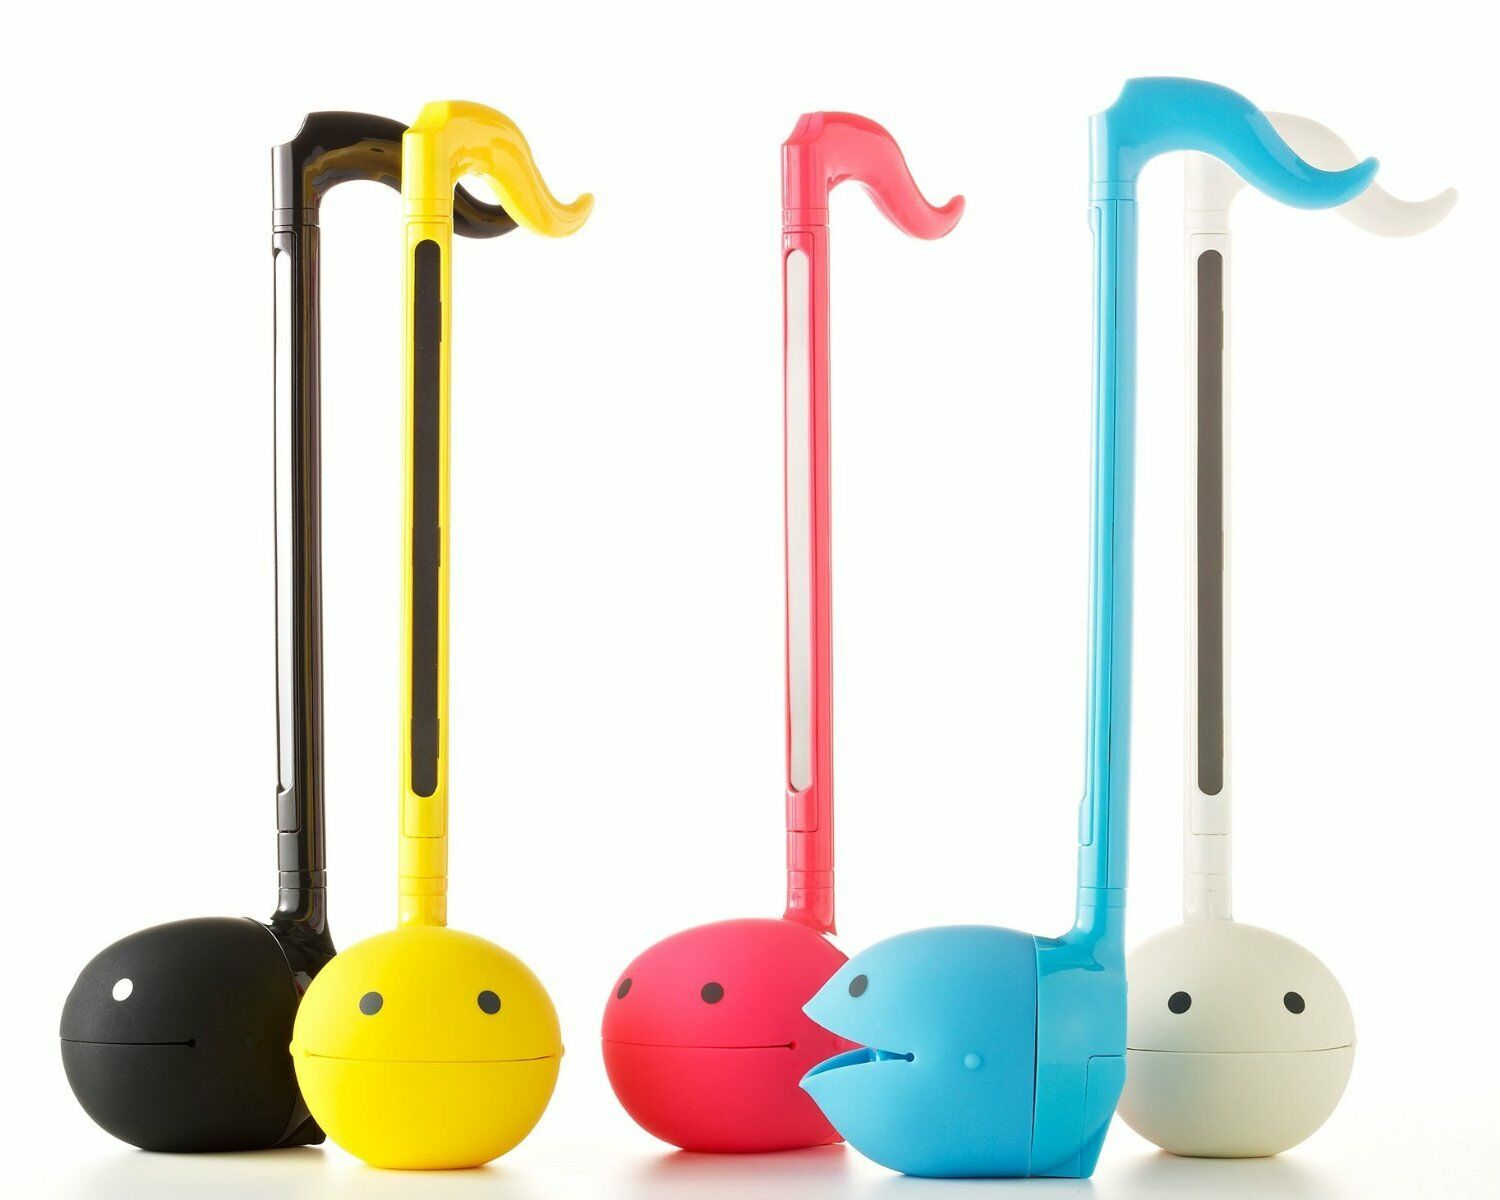
\includegraphics[width=0.8\textwidth]{otamatone.jpg}
    \end{figure}
\end{frame}

\begin{frame}{Control Interfaces - Taxonomy}
    \href{https://www.youtube.com/watch?v=PICmdczYowM}{Eyeharp}
    \begin{figure}[h]
        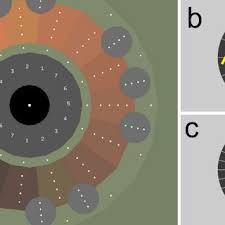
\includegraphics[width=0.6\textwidth]{eyeharp.jpeg}
    \end{figure}
\end{frame}

\begin{frame}{Control Interfaces - Taxonomy}
    \href{https://www.youtube.com/watch?v=G6H1J2k--5I}{Myo}
    \begin{figure}[h]
        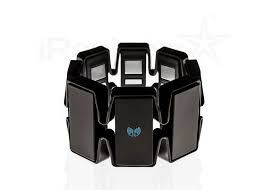
\includegraphics[width=0.9\textwidth]{myo.jpeg}
    \end{figure}
\end{frame}


\begin{frame}{Control Interfaces - Taxonomy}
    \href{https://www.youtube.com/watch?v=7YyNrtKTjnA}{EEG}
    \begin{figure}[h]
        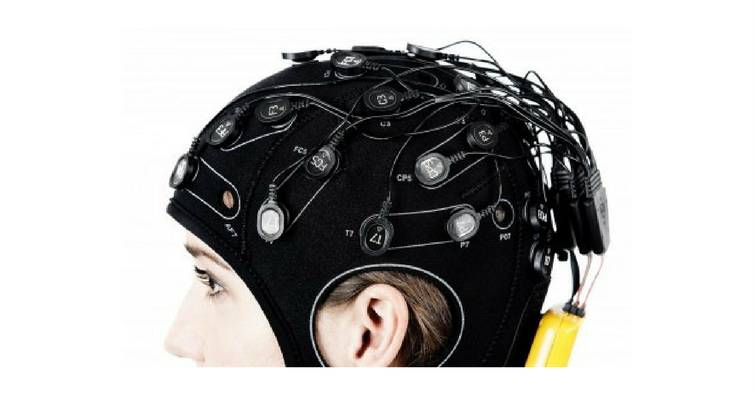
\includegraphics[width=\textwidth]{eeg.png}\blfootnote{Imotions, https://imotions.com/products/hardware/eeg-headsets/}
    \end{figure}
\end{frame}

\begin{frame}{Control Interfaces - Taxonomy}
    \href{https://www.youtube.com/watch?v=vm_FzLya8y4}{Reactable}
    \begin{figure}[h]
        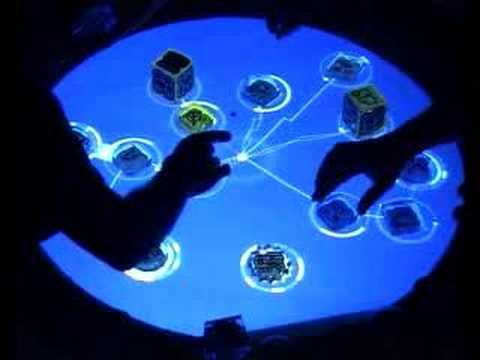
\includegraphics[width=0.8\textwidth]{reactable.jpg}
    \end{figure}
\end{frame}


\begin{frame}{Control Interfaces - Taxonomy}
    Computers as DMI interfaces?
    \begin{itemize}
        \item \href{https://www.youtube.com/watch?v=Tjf-NJNfOP4}{Live Coding}
        \item \href{https://www.youtube.com/watch?v=YSnb4beoSy4}{Mierdofón}
    \end{itemize}
\end{frame}

\begin{frame}{Control Interfaces - Taxonomy}
    \href{https://www.youtube.com/watch?v=yT50Q_Zbf3s}{Mars InSight?}
    \begin{figure}[h]
        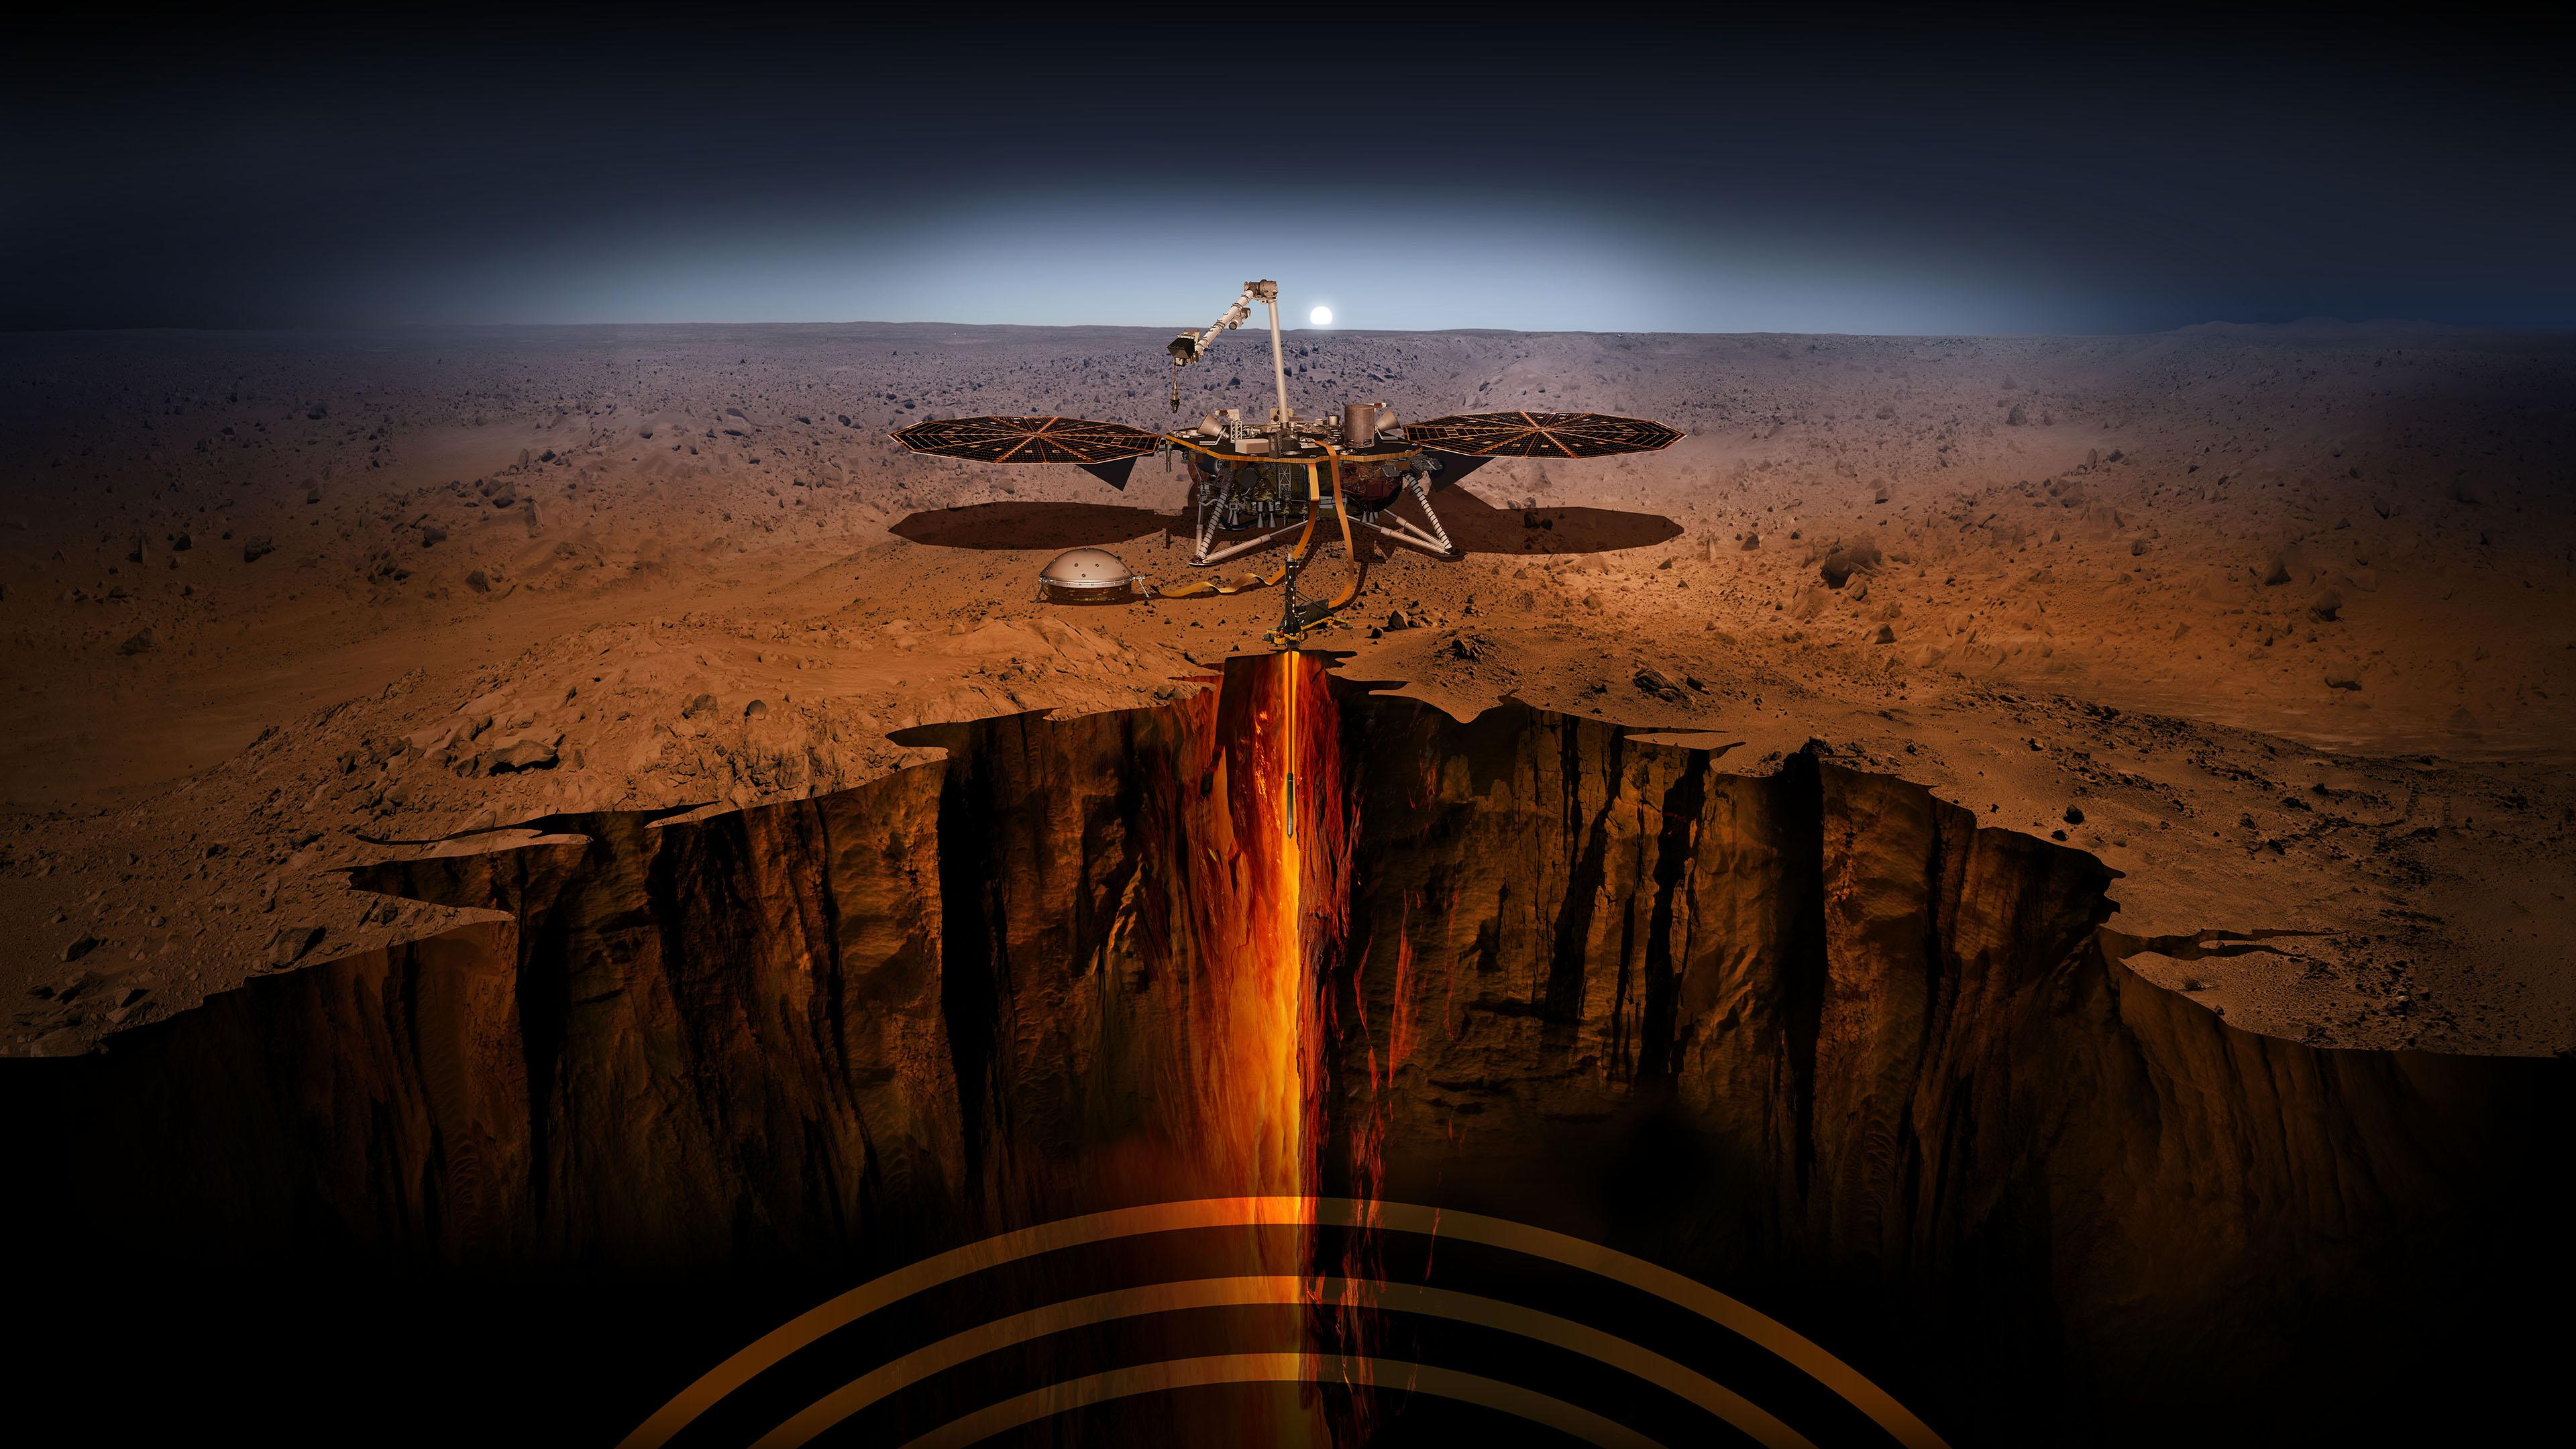
\includegraphics[width=\textwidth]{insight.jpg}
    \end{figure}
\end{frame}

%%%%%%%%%%%%%%%%%%%%%%%%%%%%%%%%%%%%%%%%%%%%%%%%%%
%%%%%%%%%%%%%%%%%%%%%%%%%%%%%%%%%%%%%%%%%%%%%%%%%%
%%%%%%%%%%%%%%%%%%%%%%%%%%%%%%%%%%%%%%%%%%%%%%%%%%
\section{Electronics}

%%%%%%%%%%%%%%%%%%%%%%%%%%%%%%%%%%%%%%%%%%%%%%%%%%
\subsection{Sensors}

\begin{frame}{Electronics - Sensors}
    "In the broadest definition, a sensor is a device, module, or subsystem whose purpose is to detect events or changes in its environment and send the information to other electronics, frequently a computer processor. A sensor is always used with other electronics."\footnote{Wikipedia, Sensors. https://en.wikipedia.org/wiki/Sensor}
\end{frame}

\begin{frame}{Electronics - Sensors}
    \textit{"Sensors are the 'sense organs of the machine'."}\footnote{Bongers, A. J. "Interaction in multimedia art." Knowledge-Based Systems 13.7-8 (2000): 479-485.}
\end{frame}

\begin{frame}{Electronics - Sensors}
    Sensors provide the way to convert measurable physical magnitudes "from our world" into quantified data understandable by a computer.
\end{frame}

\begin{frame}{Electronics - Sensors}
    DMI context: Vertegaal's sensor classification:\footnote{Vertegaal, Roel, Tamas Ungvary, and Michael Kieslinger. "Towards a musician's cockpit: Transducers, feedback and musical function." ICMC. Vol. 96. 1996.}
    \begin{itemize}
        \item Physical property sensed
        \item Resolution of sensing
        \item Direction of sensing
        \item Type and amount of feedback provided
    \end{itemize}
\end{frame}

\begin{frame}{Electronics - Sensors}
    \begin{figure}[h]
        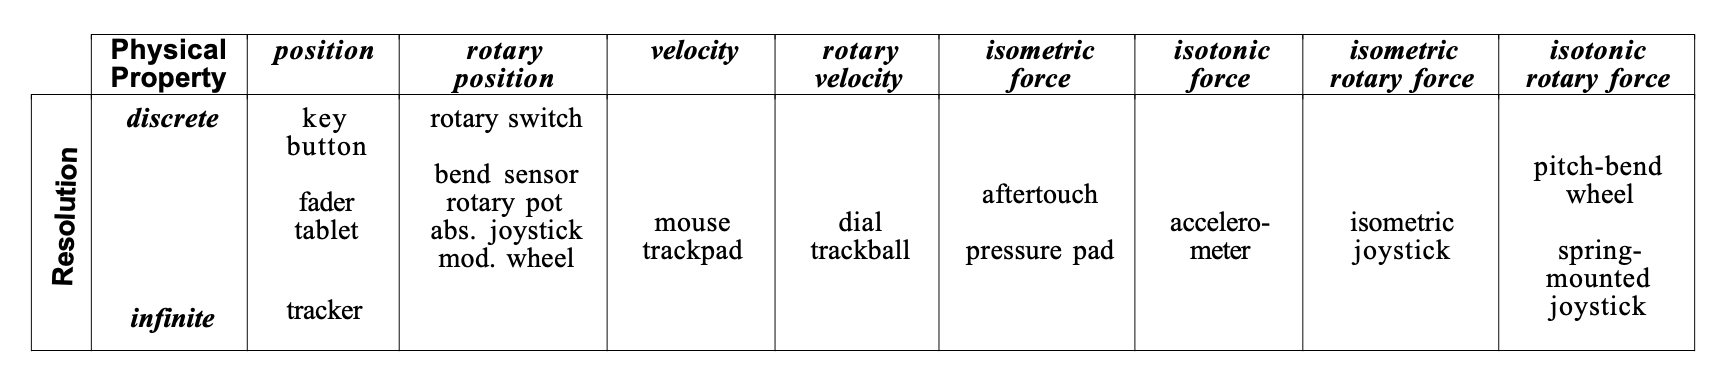
\includegraphics[width=\textwidth]{vertegaal.png}\blfootnote{from Vertegaal, Roel, Tamas Ungvary, and Michael Kieslinger. "Towards a musician's cockpit: Transducers, feedback and musical function." ICMC. Vol. 96. 1996.}
    \end{figure}
\end{frame}

\begin{frame}{Electronics - Sensors}
    \href{https://www.sparkfun.com/products/13959}{Ultrasonic Distance Sensor HC-SR04}
    \begin{figure}[h]
        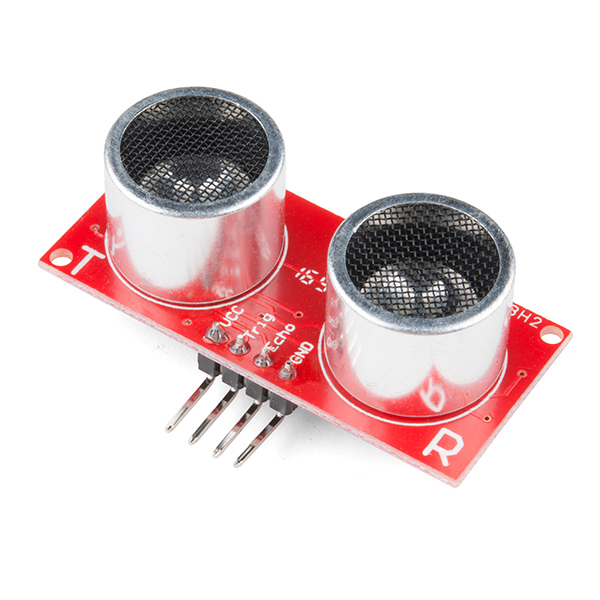
\includegraphics[width=0.75\textwidth]{ultrasonic.jpg}
    \end{figure}
\end{frame}

\begin{frame}{Electronics - Sensors}
    \href{https://www.sparkfun.com/products/10988}{Temperature Sensor TMP36}
    \begin{figure}[h]
        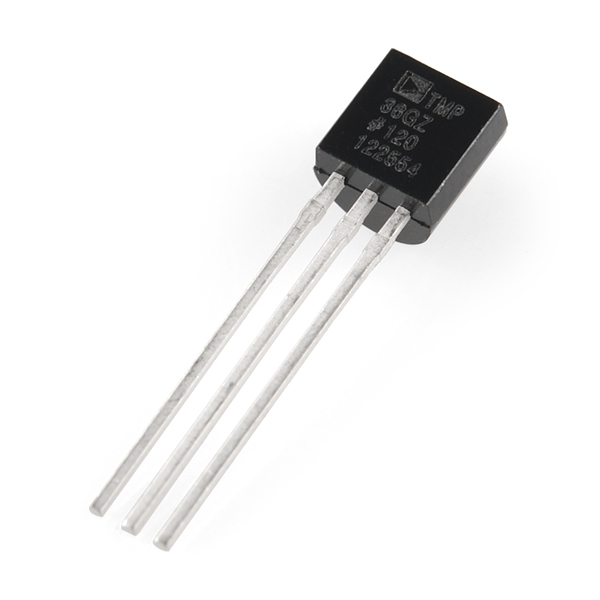
\includegraphics[width=0.75\textwidth]{temperature.jpg}
    \end{figure}
\end{frame}

\begin{frame}{Electronics - Sensors}
    \href{https://www.sparkfun.com/products/9088}{Photocell GL5528}
    \begin{figure}[h]
        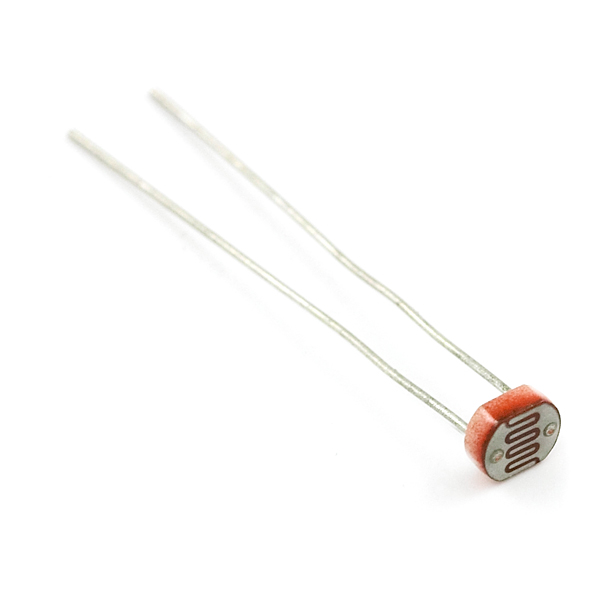
\includegraphics[width=0.75\textwidth]{photocell.jpg}
    \end{figure}
\end{frame}

\begin{frame}{Electronics - Sensors}
    \href{https://www.sparkfun.com/products/10302}{Button}
    \begin{figure}[h]
        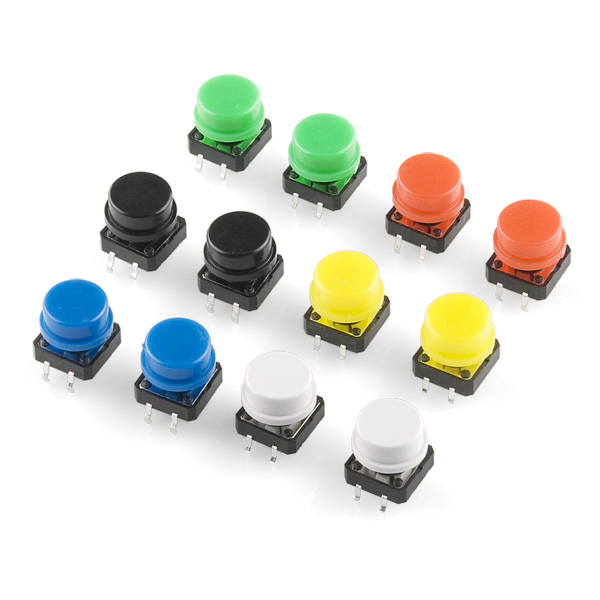
\includegraphics[width=0.75\textwidth]{buttons.jpg}
    \end{figure}
\end{frame}

\begin{frame}{Electronics - Sensors}
    \href{https://www.sparkfun.com/products/9806}{Trimpot}
    \begin{figure}[h]
        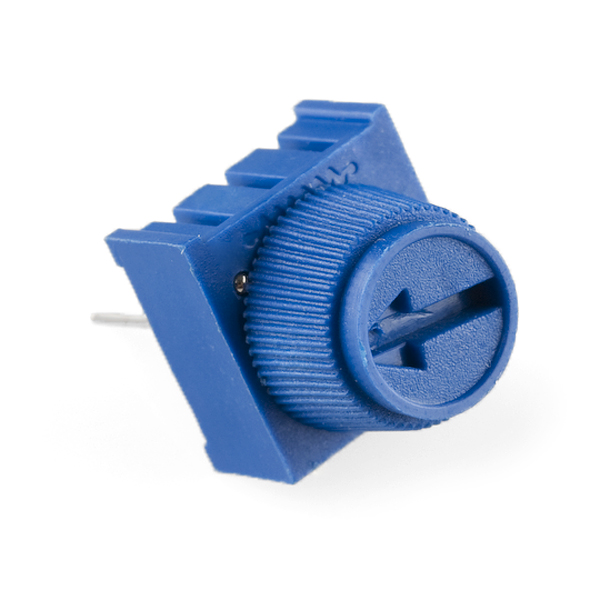
\includegraphics[width=0.75\textwidth]{trimpot.jpg}
    \end{figure}
\end{frame}

\begin{frame}{Electronics - Sensors}
    \href{https://www.sparkfun.com/products/246}{Optical Detector / Phototransistor QRD1114}
    \begin{figure}[h]
        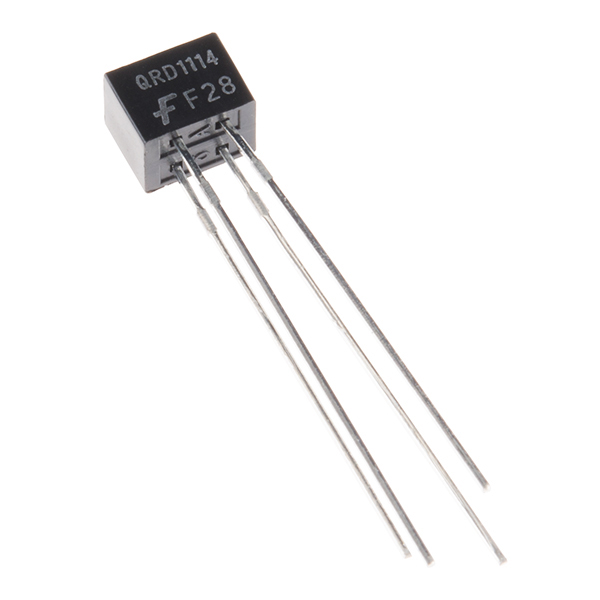
\includegraphics[width=0.75\textwidth]{optical.jpg}
    \end{figure}
\end{frame}

\begin{frame}{Electronics - Sensors}
    \href{https://www.sparkfun.com/products/8606}{Flex Sensor FS7548}
    \begin{figure}[h]
        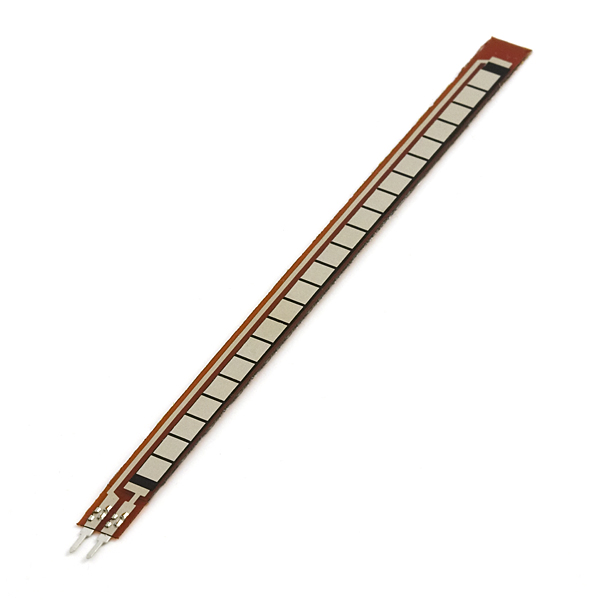
\includegraphics[width=0.75\textwidth]{flex.jpg}
    \end{figure}
\end{frame}

\begin{frame}{Electronics - Sensors}
    \href{https://www.sparkfun.com/products/8642}{Reed Switch}
    \begin{figure}[h]
        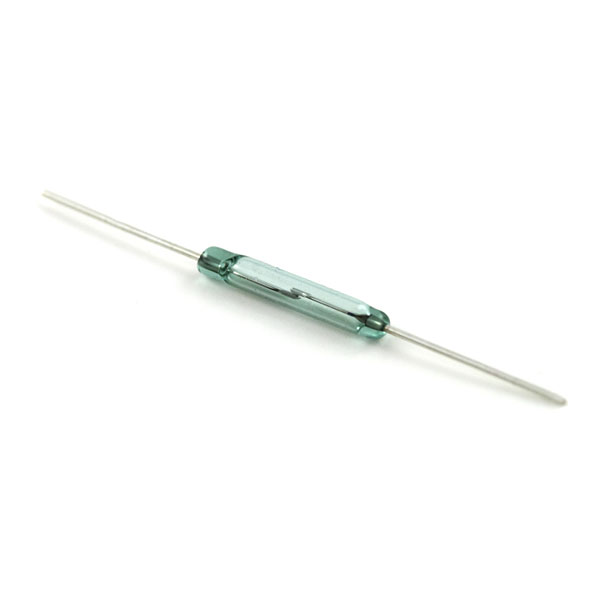
\includegraphics[width=0.75\textwidth]{reed.jpg}
    \end{figure}
\end{frame}

\begin{frame}{Electronics - Sensors}
    \href{https://www.sparkfun.com/products/8680}{Softpot Membrane Potentiometer}
    \begin{figure}[h]
        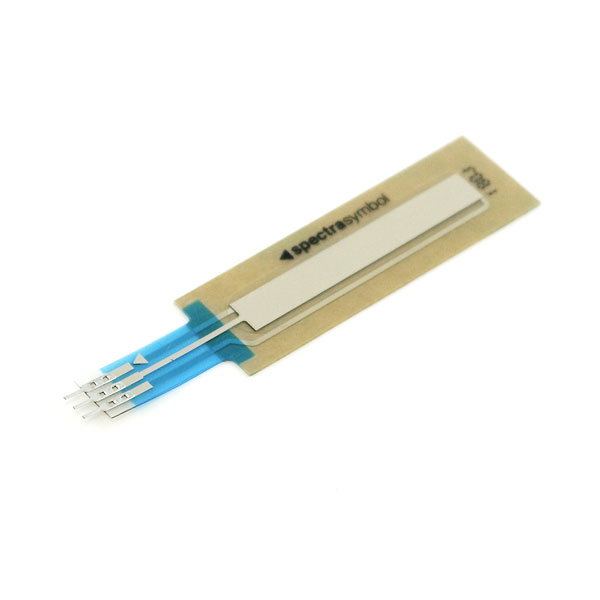
\includegraphics[width=0.75\textwidth]{softpot.jpg}
    \end{figure}
\end{frame}

\begin{frame}{Electronics - Sensors}
    \href{https://www.sparkfun.com/products/9197}{Piezo Vibration Sensor}
    \begin{figure}[h]
        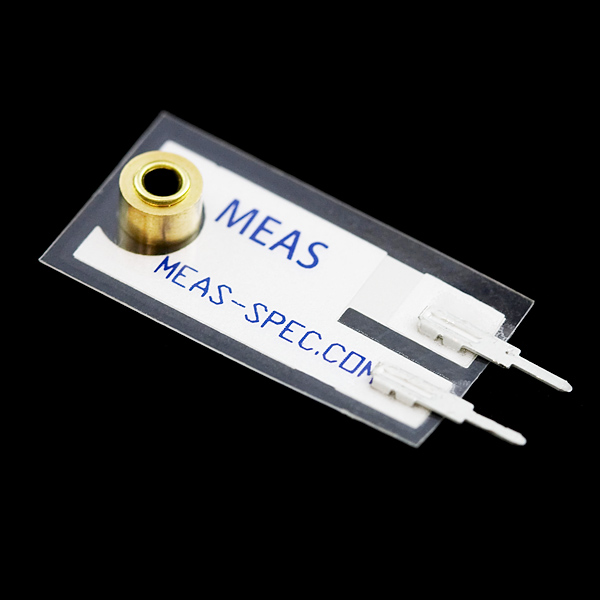
\includegraphics[width=0.65\textwidth]{piezovibration.jpg}
    \end{figure}
\end{frame}

\begin{frame}{Electronics - Sensors}
    \href{https://www.sparkfun.com/products/12787}{RGB and Gesture Sensor - APDS-9960}
    \begin{figure}[h]
        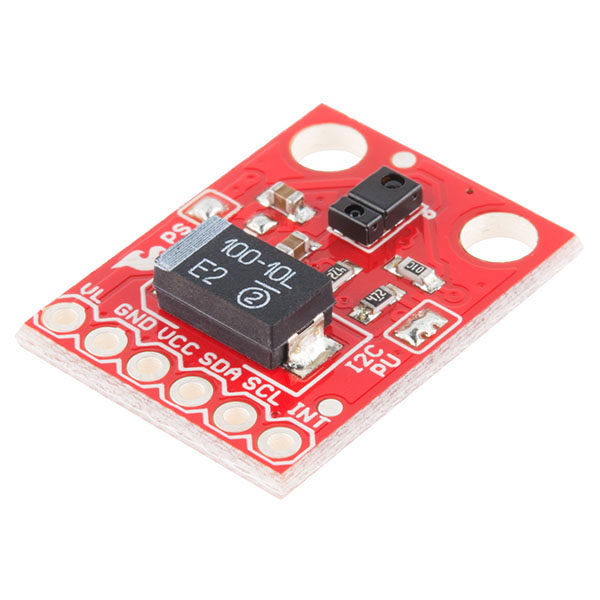
\includegraphics[width=0.75\textwidth]{rgb.jpg}
    \end{figure}
\end{frame}

\begin{frame}{Electronics - Sensors}
    \href{https://www.sparkfun.com/products/13284}{9DoF IMU Breakout - LSM9DS1}
    \begin{figure}[h]
        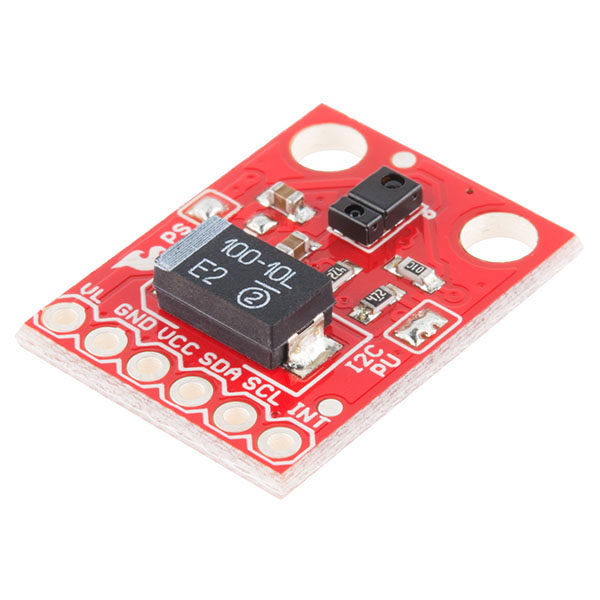
\includegraphics[width=0.75\textwidth]{rgb.jpg}
    \end{figure}
\end{frame}

\begin{frame}{Electronics - Sensors}
    \href{https://www.sparkfun.com/products/9032}{Thumb Joystick}
    \begin{figure}[h]
        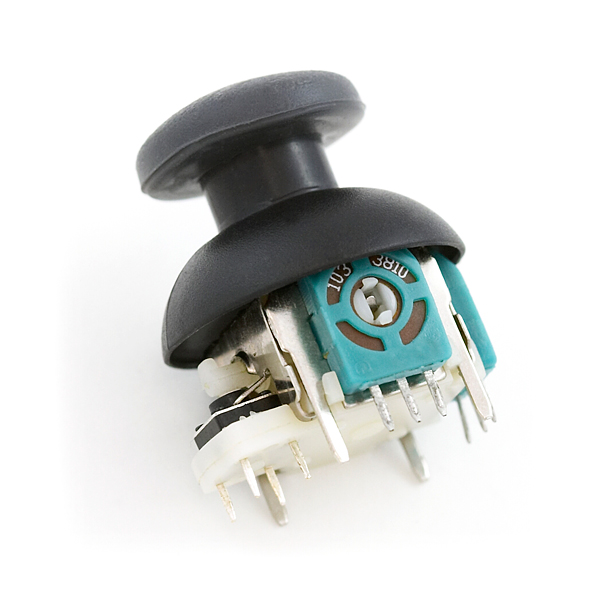
\includegraphics[width=0.75\textwidth]{joystick.jpg}
    \end{figure}
\end{frame}


%%%%%%%%%%%%%%%%%%%%%%%%%%%%%%%%%%%%%%%%%%%%%%%%%%
\subsection{Basics}

\begin{frame}{Electronics - Basics}
    \textit{"Electronics, branch of physics and electrical engineering that deals with the emission, behaviour, and effects of electrons and with electronic devices."}\footnote{"electronics | Devices, Facts, \& History". Encyclopedia Britannica. Acessed on 19/02/2019.}
\end{frame}

\begin{frame}{Electronics - Basics}
    Three fundamental physical magnitudes:
    \begin{itemize}
        \item Voltage (V) \\Electric potential difference. Measured in \textit{Volts (V).}
        \item Current (I)\\Amount of transmitted charge per surface and time unit.  Measured in \textit{Amperes (A).}
        \item Resistance (R) / Impedance (Z) \\Opposition to the electrical flow. Measured in \textit{Ohms ($\Omega$).}
    \end{itemize}
\end{frame}

\begin{frame}{Electronics - Basics}
    Hydraulic analogy\footnote{Wikipedia. Hydraulic analogy. https://en.wikipedia.org/wiki/Hydraulic\_analogy. Accessed 19/02/2019}:
    \begin{itemize}
        \item Voltage / Gravitational Potential
        \item Current / Flow Rate
        \item Resistance / Pipe constriction
    \end{itemize}
\end{frame}

\begin{frame}{Electronics - Basics}
    Ohm's Law\\
    $V = IR$
    \begin{figure}[h]
        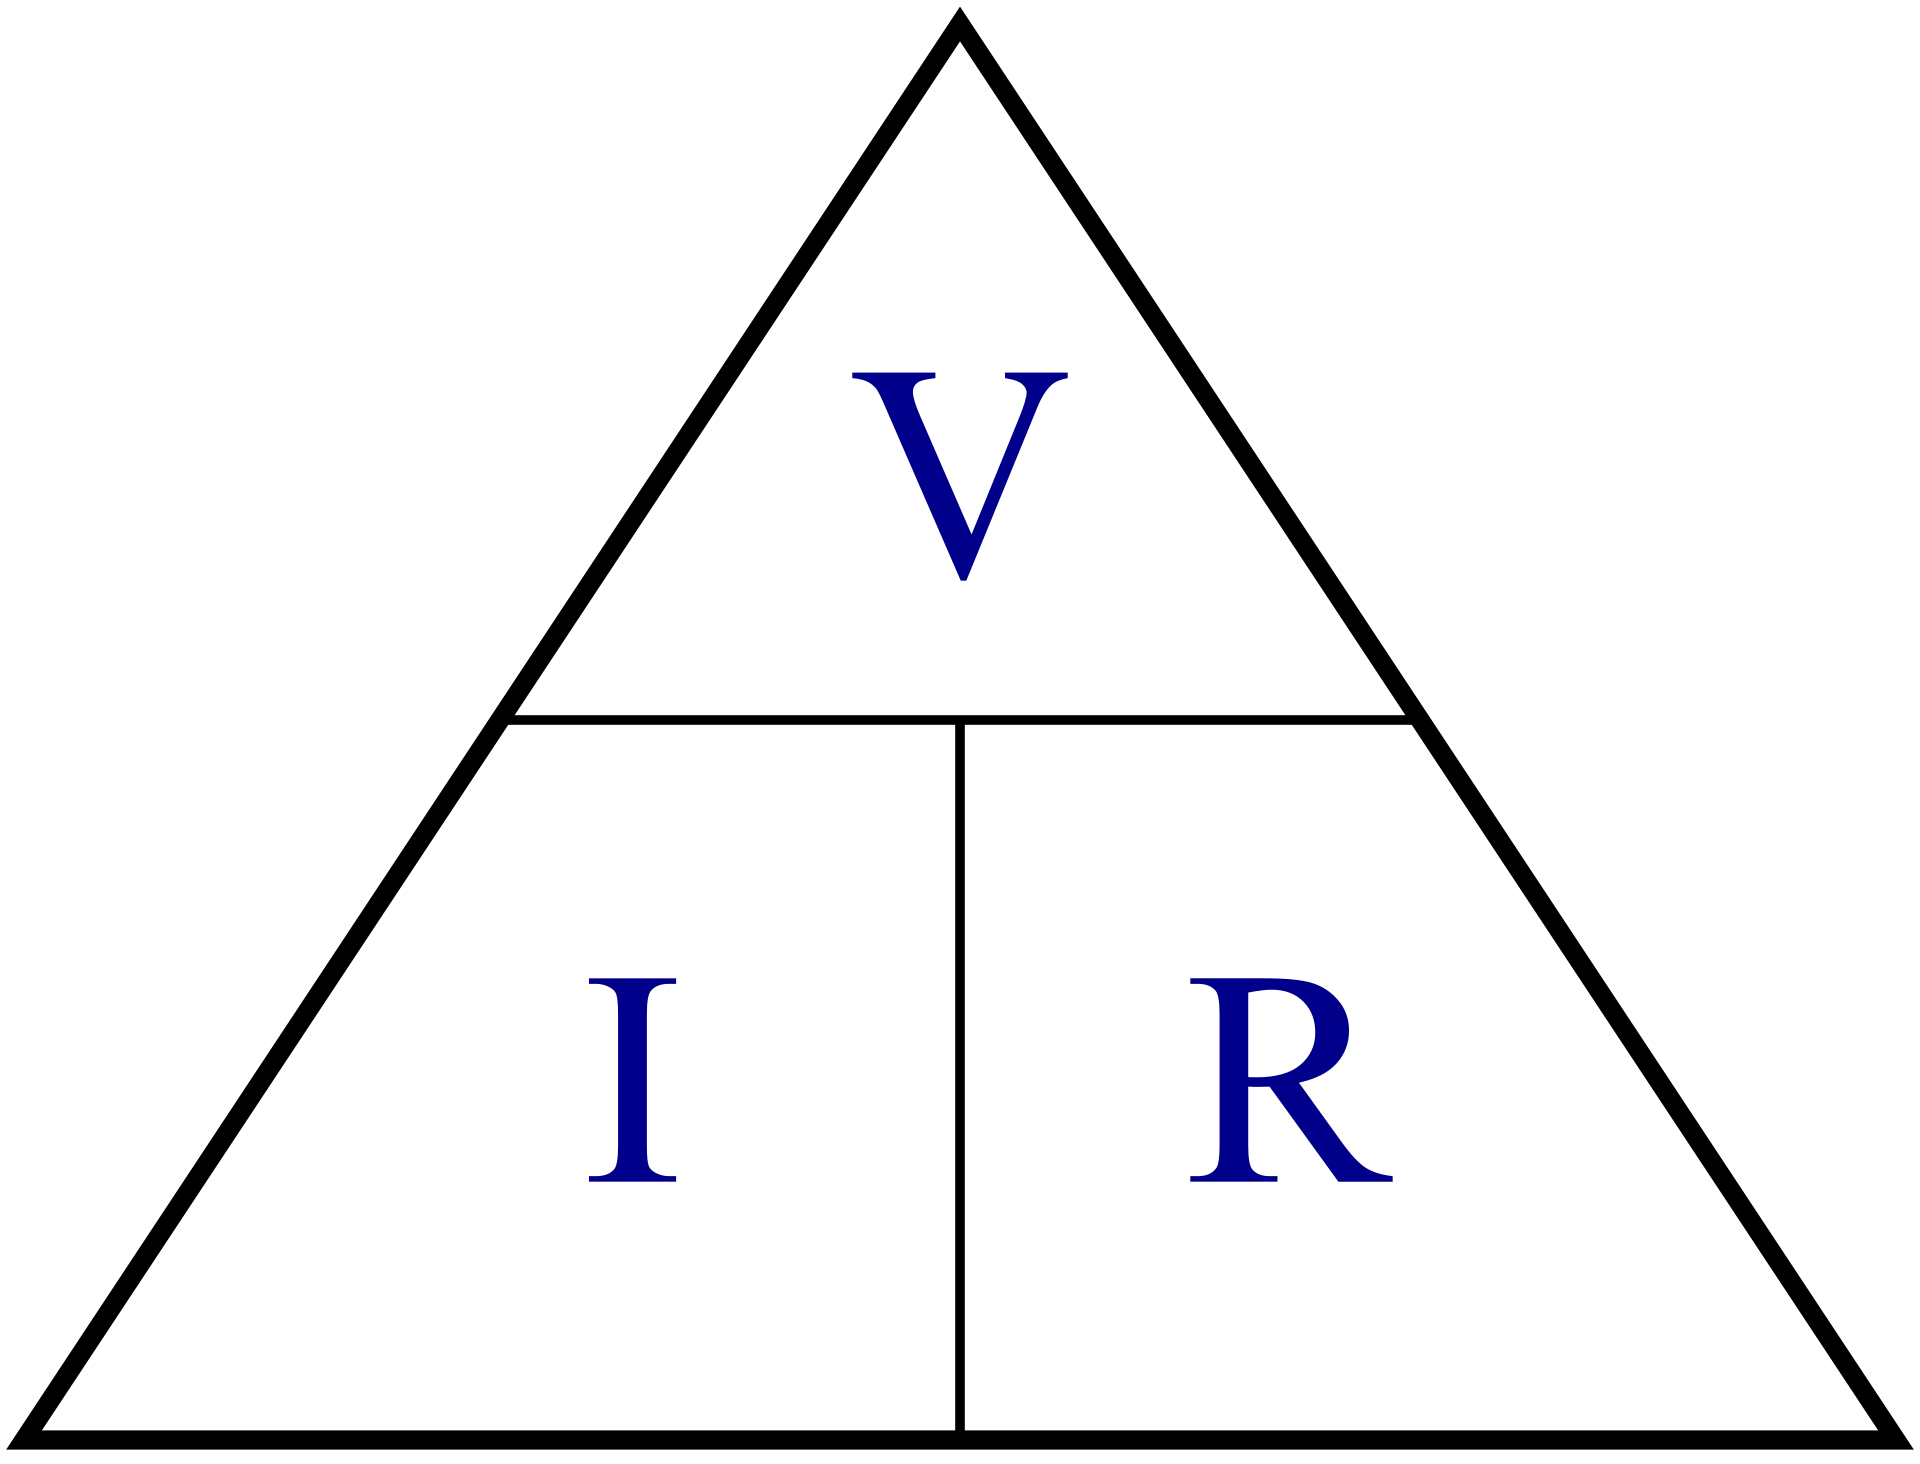
\includegraphics[width=0.75\textwidth]{ohm.png}
    \end{figure}
\end{frame}

\begin{frame}{Electronics - Basics}
    \begin{figure}[h]
        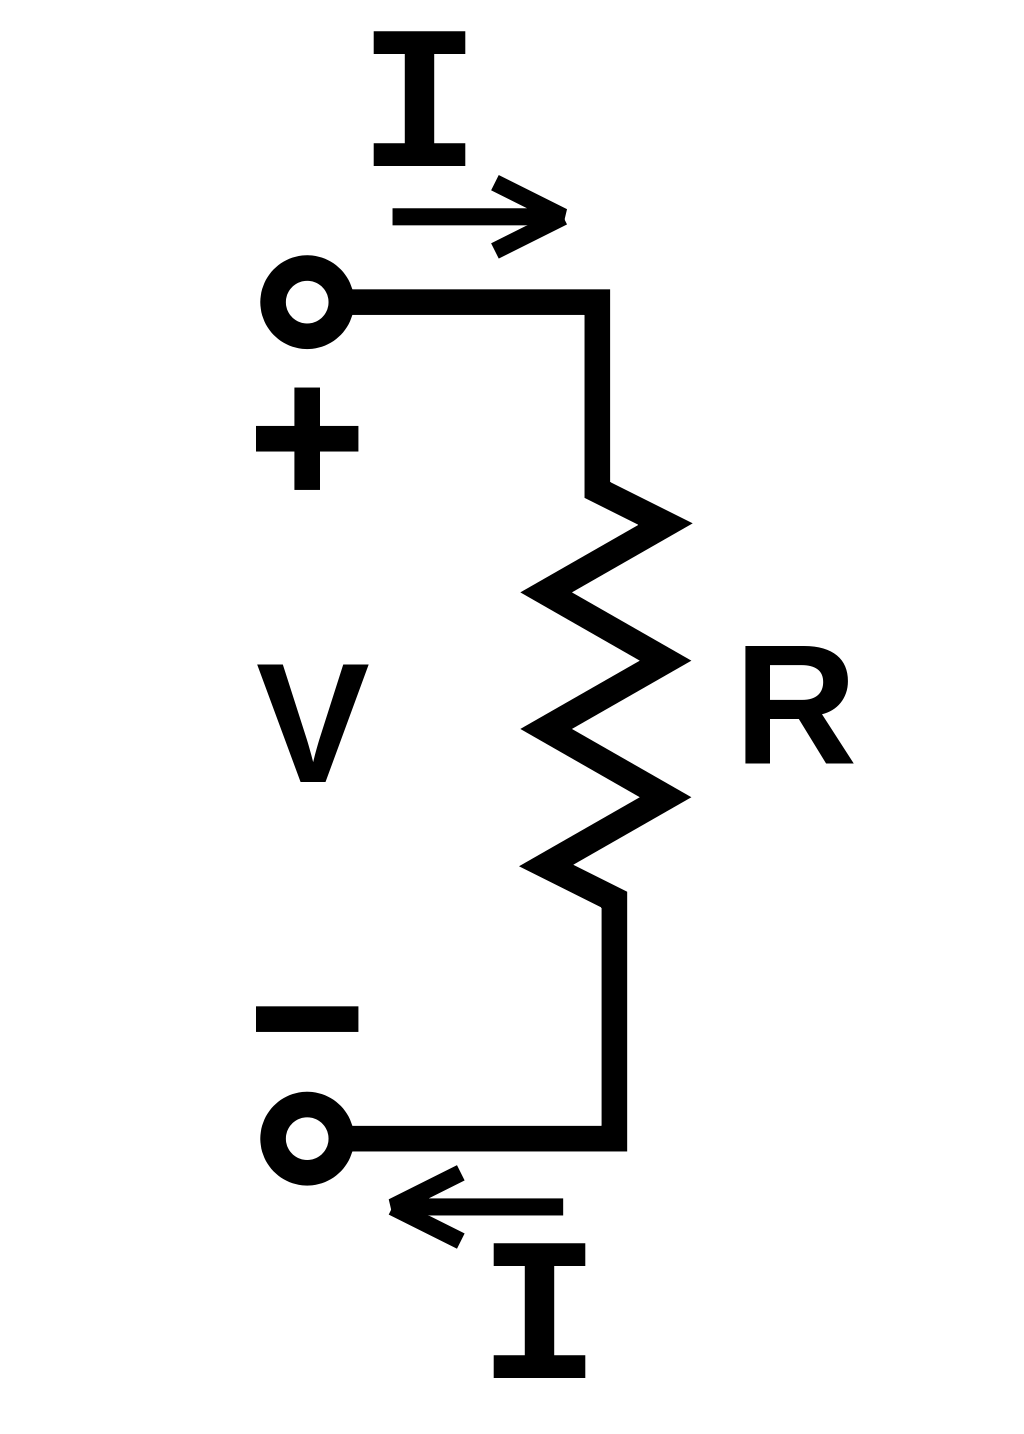
\includegraphics[width=0.5\textwidth]{electronics.png}
    \end{figure}
\end{frame}

\begin{frame}{Electronics - Basics}
    Combining impedances\\
    \vspace{5mm}
    Series:\blfootnote{By Omegatron - This W3C-unspecified circuit diagram was created with the Electrical Symbols Library, CC BY-SA 3.0, https://commons.wikimedia.org/w/index.php?curid=2049108}
    \begin{figure}[h]
        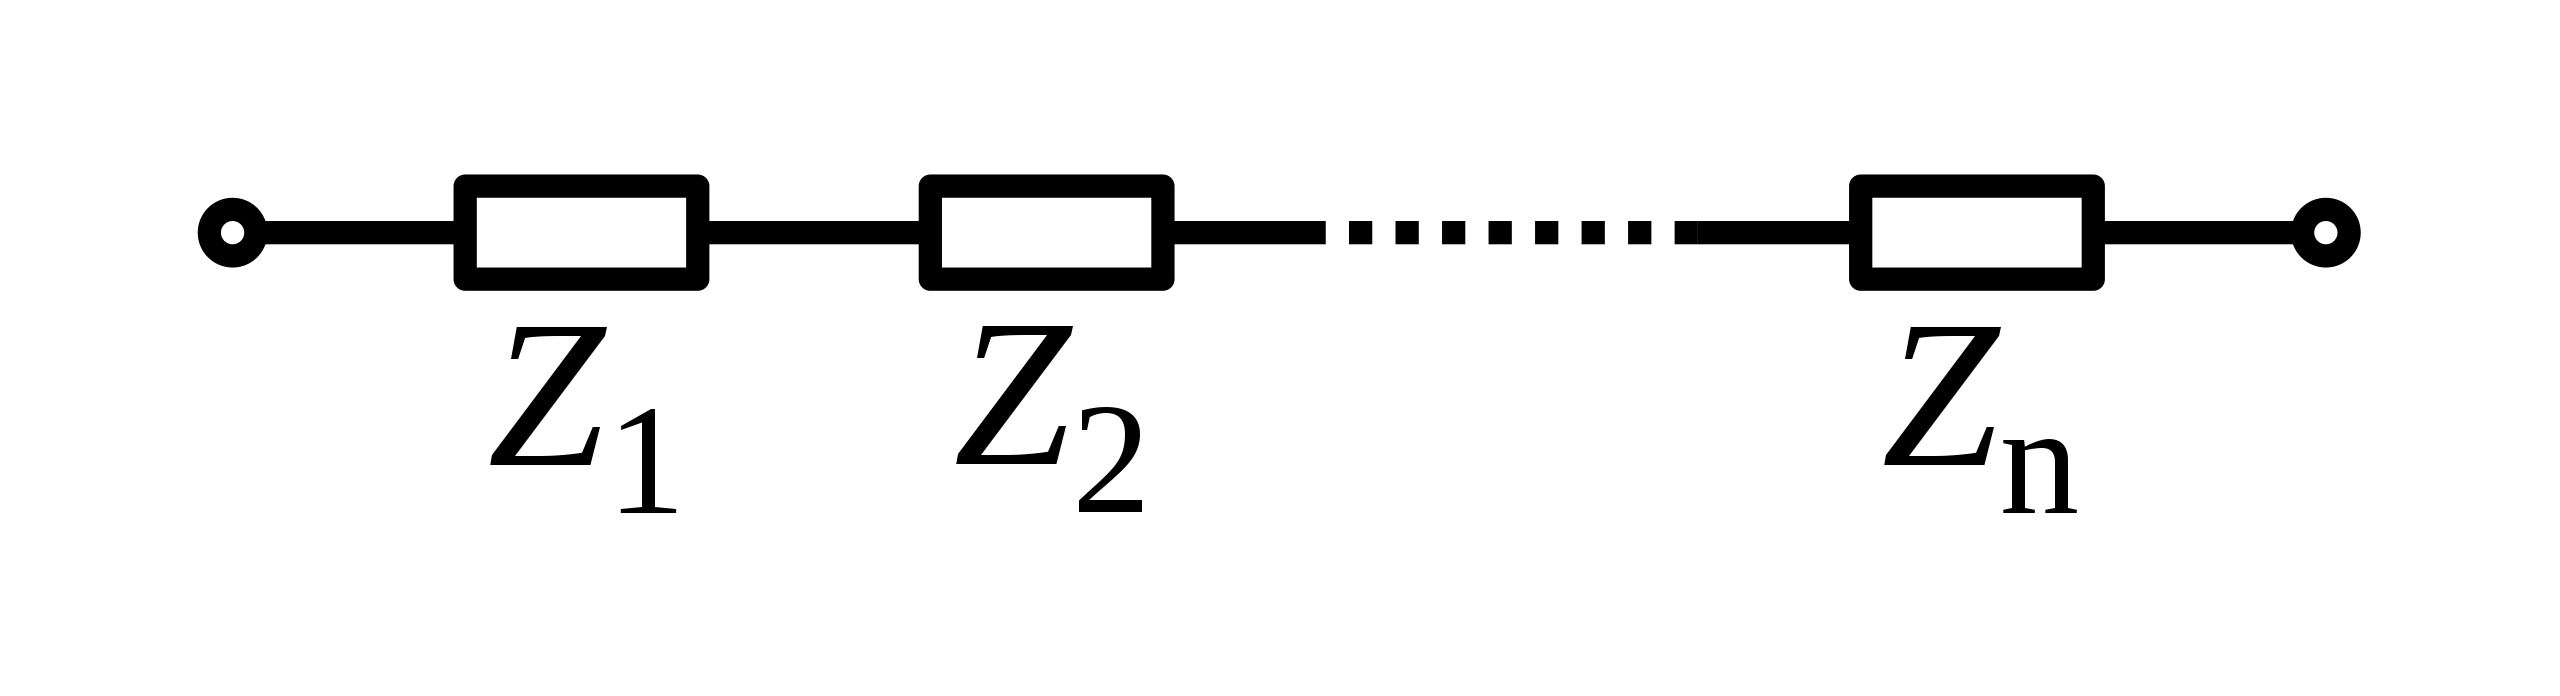
\includegraphics[width=0.5\textwidth]{series.png}
    \end{figure}
    \begin{equation*}
        \Large
        Z_{eq} = Z_1 + Z_2 + ... + Z_N
    \end{equation*}
\end{frame}

\begin{frame}{Electronics - Basics}
    Combining impedances\\
    \vspace{5mm}
    Parallel:\blfootnote{By Omegatron - This W3C-unspecified circuit diagram was created with the Electrical Symbols Library, CC BY-SA 3.0, https://commons.wikimedia.org/w/index.php?curid=2049107}
    \begin{figure}[h]
        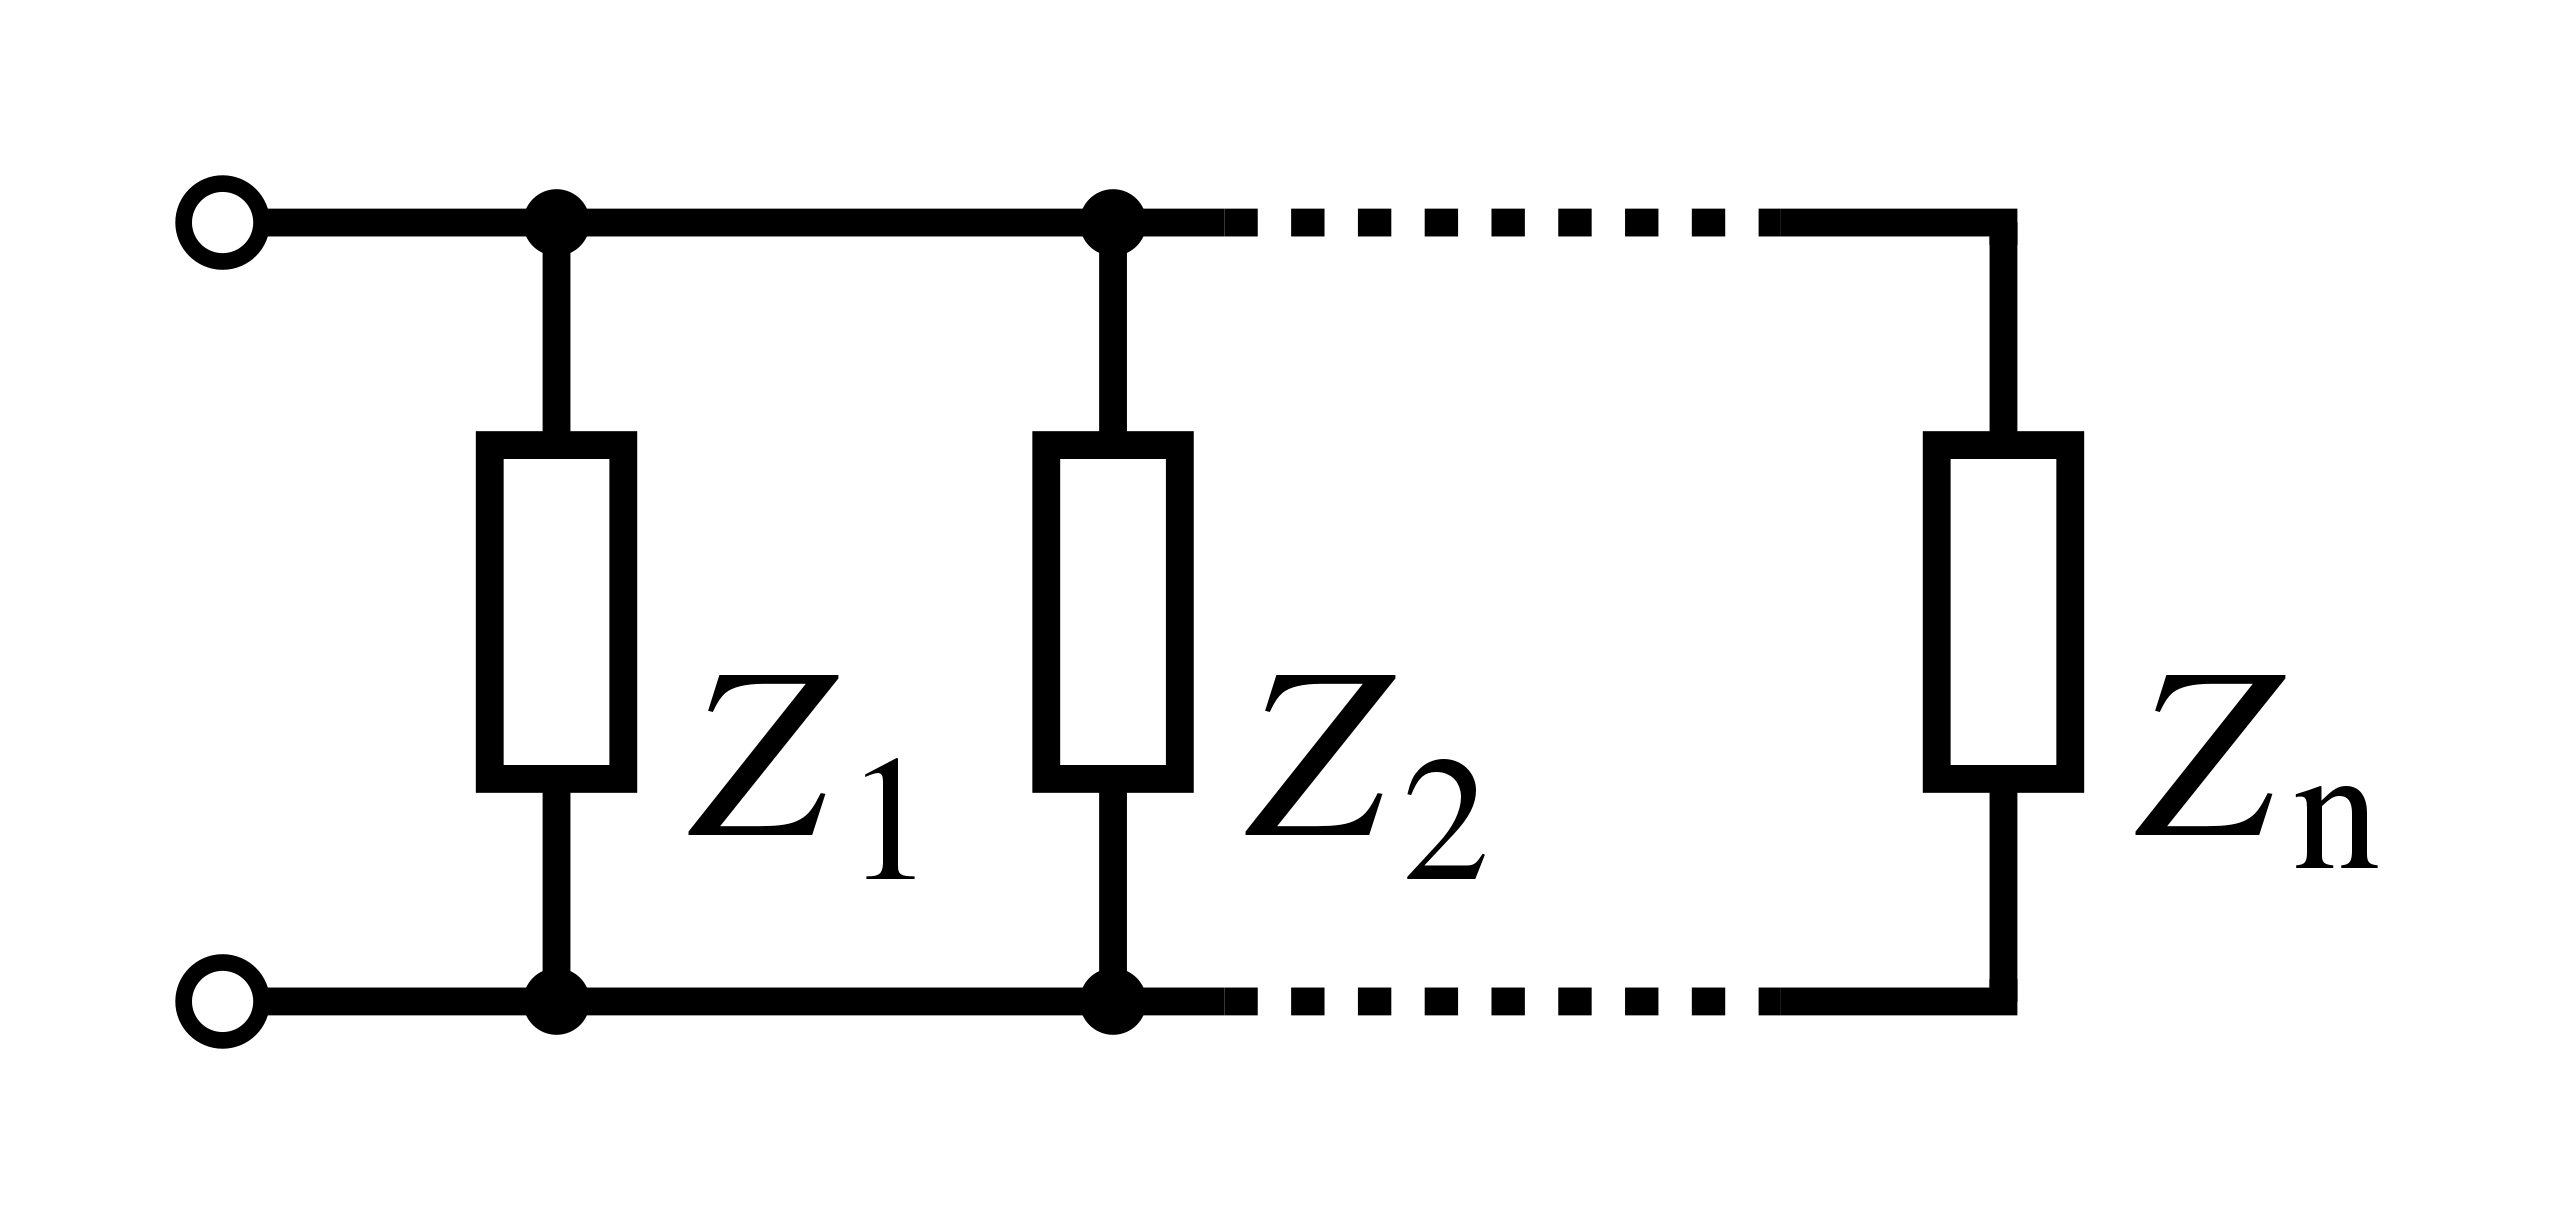
\includegraphics[width=0.5\textwidth]{parallel.png}
    \end{figure}
    \begin{equation*}
        \Large
        \frac{1}{Z_{eq}} = \frac{1}{Z_1} + \frac{1}{Z_2} + ... + \frac{1}{Z_N}
    \end{equation*}
\end{frame}

\begin{frame}{Electronics - Basics}
    Voltage Divider\blfootnote{By Velociostrich - Own work, CC BY-SA 3.0, https://commons.wikimedia.org/w/index.php?curid=7765066}\\
    \vspace{5mm}
    \begin{figure}[h]
        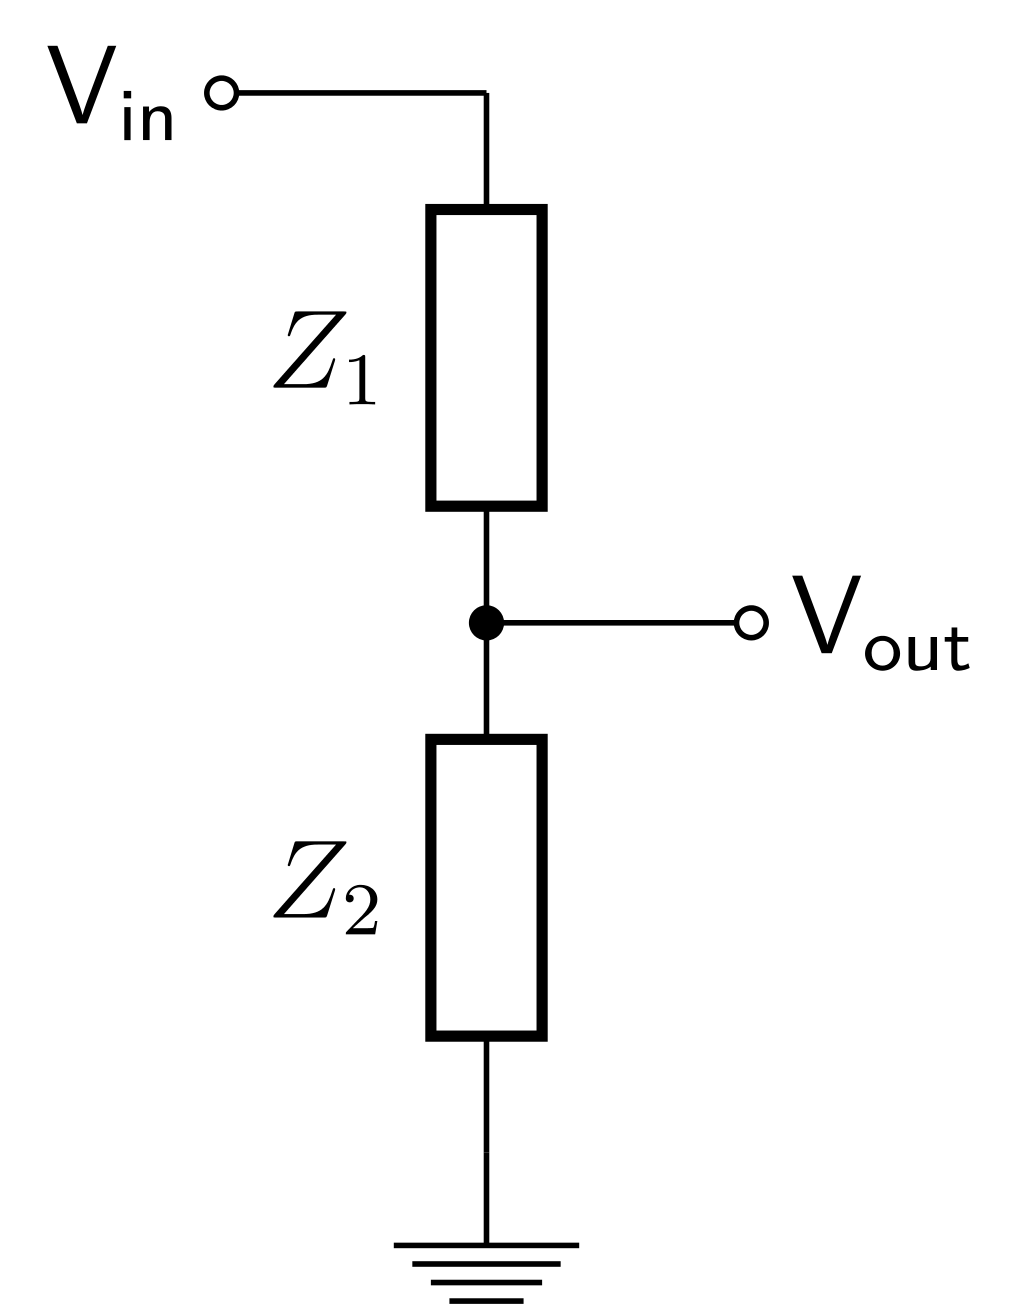
\includegraphics[width=0.25\textwidth]{voltage_divider.png}
    \end{figure}
    \begin{equation*}
    \Large
        V_{out} = \frac{Z_2}{Z_1+Z_2}V_{in}
    \end{equation*}
\end{frame}

\begin{frame}{Electronics - Basics}
   Resistor Color Chart\blfootnote{Digi-Key, 4 Band Resistor Color Code Calculator. https://www.digikey.com/en/resources/conversion-calculators/conversion-calculator-resistor-color-code-4-band.}\\
    \vspace{5mm}
    \begin{figure}[h]
        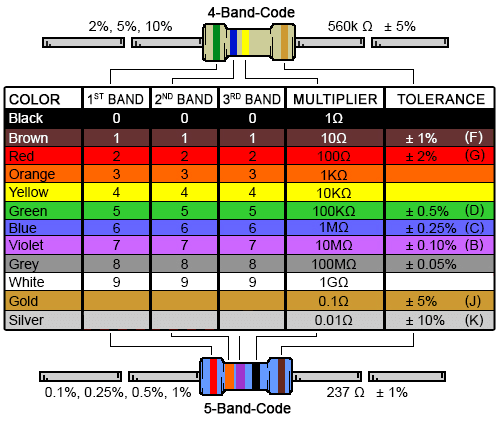
\includegraphics[width=0.6\textwidth]{resistor-color-chart.png}
    \end{figure}
\end{frame}

\begin{frame}{Electronics - Basics}
   \textit{"\textbf{Arduino} is an open-source electronics platform based on easy-to-use hardware and software. It's intended for anyone making interactive projects."}\footnote{https://www.arduino.cc/}
    \vspace{5mm}
    \begin{figure}[h]
        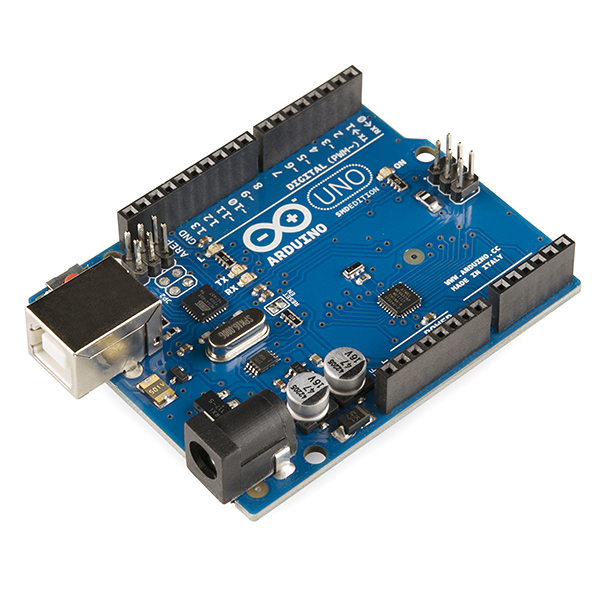
\includegraphics[width=0.5\textwidth]{arduino.jpg}
    \end{figure}
\end{frame}







\end{document}
